\documentclass{oblivoir}
%%%Default packages
\usepackage{amsmath,amssymb,amsthm,kotex,tabu,graphicx,pifont}
\usepackage{../kswrapfig}

\usepackage{gensymb} %\degree

%%%More packages
%\usepackage{caption,subcaption}
%\usepackage[perpage]{footmisc}
%
\usepackage[skipabove=10pt,innertopmargin=10pt,nobreak=true]{mdframed}

\usepackage[inline]{enumitem}
\setlist[enumerate,1]{label=(\arabic*)}
\setlist[enumerate,2]{label=(\alph*)}

\usepackage{multicol}
\setlength{\columnsep}{30pt}
\setlength{\columnseprule}{1pt}
%
%\usepackage{forest}
%\usetikzlibrary{shapes.geometric,arrows.meta,calc}
%
%%%defi theo exam prob rema proo
%이 환경들 아래에 문단을 쓸 경우 살짝 들여쓰기가 되므로 \hspace{-.7em}가 필요할 수 있다.

\newcounter{num}
\newcommand{\defi}[1]
{\noindent\refstepcounter{num}\textbf{정의 \arabic{num})} #1\par\noindent}
\newcommand{\theo}[1]
{\noindent\refstepcounter{num}\textbf{정리 \arabic{num})} #1\par\noindent}
\newcommand{\revi}[1]
{\noindent\refstepcounter{num}\textbf{복습 \arabic{num})} #1\par\noindent}
\newcommand{\exam}[1]
{\bigskip\bigskip\noindent\refstepcounter{num}\textbf{예시 \arabic{num})} #1\par\noindent}
\newcommand{\prob}[1]
{\bigskip\bigskip\noindent\refstepcounter{num}\textbf{문제 \arabic{num})} #1\par\noindent}
\newcommand{\rema}[1]
{\bigskip\bigskip\noindent\refstepcounter{num}\textbf{참고 \arabic{num})} #1\par\noindent}
\newcommand{\proo}
{\bigskip\noindent\textsf{증명)}}

\newenvironment{talign}
 {\let\displaystyle\textstyle\align}
 {\endalign}
\newenvironment{talign*}
 {\let\displaystyle\textstyle\csname align*\endcsname}
 {\endalign}
%
%%%Commands

\newcommand{\procedure}[1]{\begin{mdframed}\vspace{#1\textheight}\end{mdframed}}

\newcommand\an[1]{\par\bigskip\noindent\textbf{문제 \ref{#1})}\par\noindent}

\newcommand\ann[2]{\par\bigskip\noindent\textbf{문제 \ref{#1})}\:\:#2\par\medskip\noindent}

\newcommand\ans[1]{\begin{flushright}\textbf{답 : }#1\end{flushright}}

\newcommand\anssec[1]{\bigskip\bigskip\noindent{\large\bfseries#1}}

\newcommand{\pb}[1]%\Phantom + fBox
{\fbox{\phantom{\ensuremath{#1}}}}

\newcommand\ba{\,|\,}

\newcommand\ovv[1]{\ensuremath{\overline{#1}}}
\newcommand\ov[2]{\ensuremath{\overline{#1#2}}}
%
%%%% Settings
%\let\oldsection\section
%
%\renewcommand\section{\clearpage\oldsection}
%
%\let\emph\textsf
%
%\renewcommand{\arraystretch}{1.5}
%
%%%% Footnotes
%\makeatletter
%\def\@fnsymbol#1{\ensuremath{\ifcase#1\or
%*\or **\or ***\or
%\star\or\star\star\or\star\star\star\or
%\dagger\or\dagger\dagger\or\dagger\dagger\dagger
%\else\@ctrerr\fi}}
%
%\renewcommand{\thefootnote}{\fnsymbol{footnote}}
%\makeatother
%
%\makeatletter
%\AtBeginEnvironment{mdframed}{%
%\def\@fnsymbol#1{\ensuremath{\ifcase#1\or
%*\or **\or ***\or
%\star\or\star\star\or\star\star\star\or
%\dagger\or\dagger\dagger\or\dagger\dagger\dagger
%\else\@ctrerr\fi}}%
%}   
%\renewcommand\thempfootnote{\fnsymbol{mpfootnote}}
%\makeatother
%
%%% 객관식 선지
\newcommand\one{\ding{172}}
\newcommand\two{\ding{173}}
\newcommand\three{\ding{174}}
\newcommand\four{\ding{175}}
\newcommand\five{\ding{176}}
\usepackage{tabto,pifont}
%\TabPositions{0.2\textwidth,0.4\textwidth,0.6\textwidth,0.8\textwidth}

\newcommand\taba[5]{\par\noindent
\one\:{#1}
\tabto{0.2\textwidth}\two\:\:{#2}
\tabto{0.4\textwidth}\three\:\:{#3}
\tabto{0.6\textwidth}\four\:\:{#4}
\tabto{0.8\textwidth}\five\:\:{#5}}

\newcommand\tabb[5]{\par\noindent
\one\:{#1}
\tabto{0.33\textwidth}\two\:\:{#2}
\tabto{0.67\textwidth}\three\:\:{#3}\medskip\par\noindent
\four\:\:{#4}
\tabto{0.33\textwidth}\five\:\:{#5}}

\newcommand\tabc[5]{\par\noindent
\one\:{#1}
\tabto{0.5\textwidth}\two\:\:{#2}\medskip\par\noindent
\three\:\:{#3}
\tabto{0.5\textwidth}\four\:\:{#4}\medskip\par\noindent
\five\:\:{#5}}

\newcommand\tabd[5]{\par\noindent
\one\:{#1}\medskip\par\noindent
\two\:\:{#2}\medskip\par\noindent
\three\:\:{#3}\medskip\par\noindent
\four\:\:{#4}\medskip\par\noindent
\five\:\:{#5}}
%
%%%% fonts
%
%\usepackage{fontspec, xunicode, xltxtra}
%\setmainfont[]{은 바탕}
%\setsansfont[]{은 돋움}
%\setmonofont[]{은 바탕}
%\XeTeXlinebreaklocale "ko"
%%%%
\begin{document}

\title{수학(하) : 10 함수}
\author{}
\date{\today}
\maketitle
\tableofcontents
\newpage

%%
\section{함수}
%
\begin{mdframed}\label{function1}
\defi{함수}
두 집합 \(X\), \(Y\)에 대하여, \(X\)의 모든 원소 \(x\)가 \(Y\)의 한 원소 \(y\)에 대응되는 것을 \fbox{함수}라고 한다.\footnotemark
\end{mdframed}
\footnotetext{이것을 기호로 \(f:X\to Y\)로 나타낸다.}
%
\exam{}
\begin{enumerate}\label{function2}
\item
다음 그림에서 각 국가를 그 국가에 속한 도시에 연결하여라.
\begin{center}
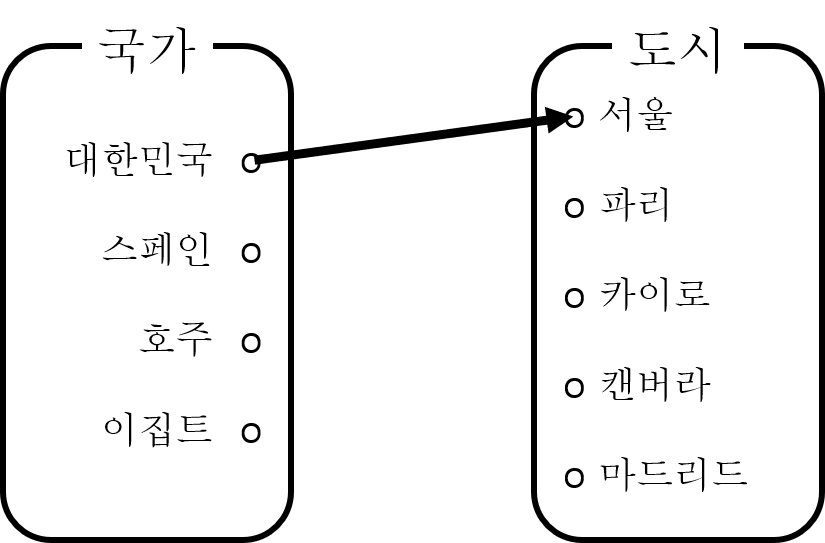
\includegraphics[width=0.4\textwidth]{function_2}
\end{center}
\item
위의 그림은 하나의 함수를 나타낸다.
집합 `국가'의 모든 원소들은\\
집합 `도시'의 한 원소에 대응되었다.
`대한민국'이 `서울'에 대응된 것을
\[f(대한민국)=서울\]
와 같이 나타내고 `서울'을 `대한민국'의 \fbox{함숫값}이라고 말한다.
마찬가지로
\(f(스페인)=\pb{마드리드}\), \(f(호주)=\pb{캔버라}\), \(f(이집트)=\pb{카이로}\)이다.
\item
집합 `국가'를 \fbox{정의역}, 집합 `도시'를 \fbox{공역}이라고 한다.
한편, 함숫값들의 집합을 \fbox{치역}이라고 한다.%
\footnote{그러므로 치역은 공역의 부분집합이다.}
따라서
\begin{align*}
정의역	&=\{대한민국,\,스페인,\,호주,\,이집트\}\\
공역		&=\{서울,\,파리,\,카이로,\,캔버라,\,마드리드\}\\
치역		&=\{서울,\,카이로,\,캔버라,\,마드리드\}
\end{align*}
\end{enumerate}

%
\prob{}\label{function3}
다음 대응들 중 함수인 것을 골라라.
\begin{center}
(1)\hspace{100pt}(2)\hspace{100pt}(3)\\
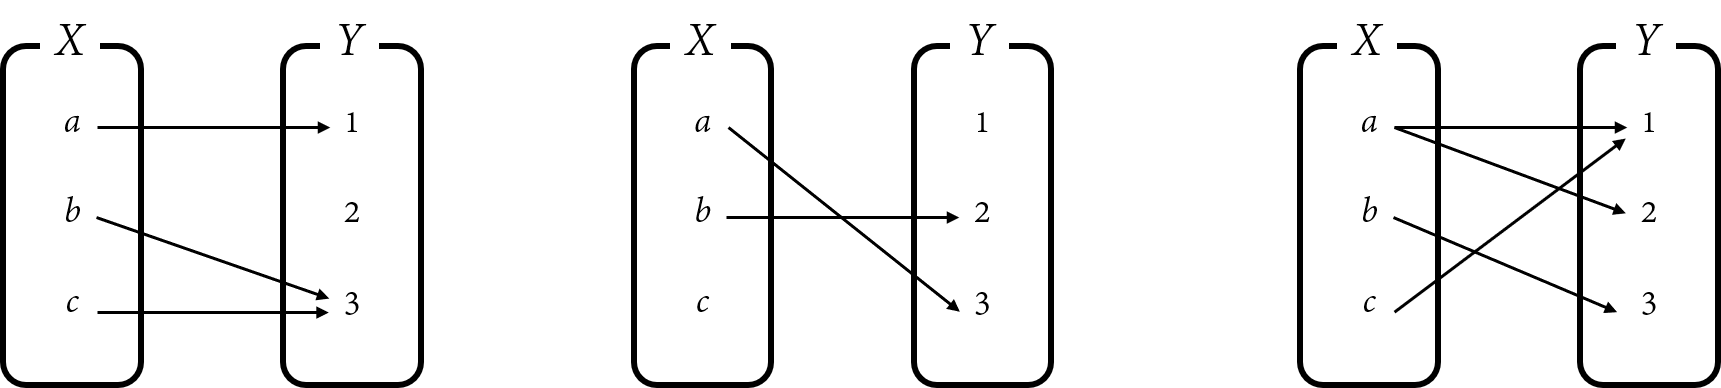
\includegraphics[width=0.9\textwidth]{function_3}
\end{center}

%
\prob{두 집합 \(X=\{1,2,3,4,5,6\}\), \(Y=\{1,2,3,4,5\}\)에 대하여}\label{function4}
함수 \(f:X\to Y\)를
\[f(x)=x\text{의 약수의 개수}\]
라고 하자.
예를 들어 \(1\)의 약수는 \(1\)개이므로 \(f(1)=1\)이다.
\begin{enumerate}
\item
다음 대응을 완성하여라.
\begin{center}
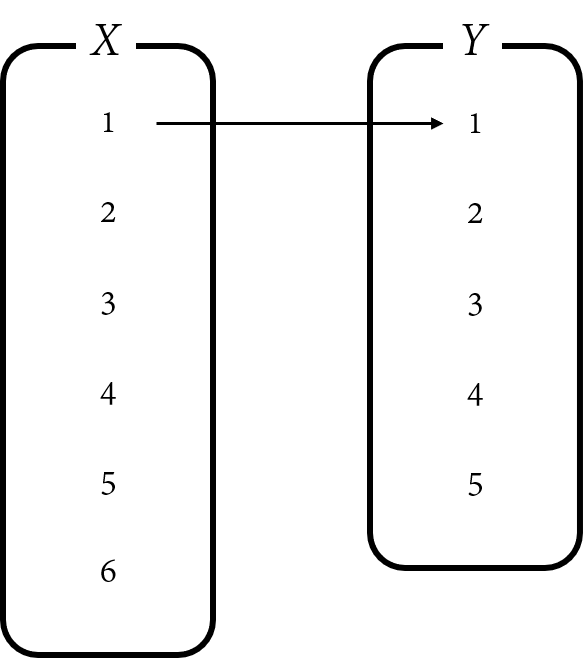
\includegraphics[width=0.27\textwidth]{function_4}
\end{center}
\item
정의역$=$\\
공역$=$\\
치역$=$
\end{enumerate}

%
\prob{두 집합 \(X=\{1,2,3,4,5,6,7,8,9,10\}\), \(Y=\{0,1,2,3\}\)에 대하여}\label{function5}
 함수 \(f:X\to Y\)를
\[f(x)=x\text{를 4로 나누었을 때의 나머지}\]
라고 하자.
이때, \(f(3)\), \(f(8)\), \(f(10)\)의 값을 차례로 구하여라.

정의역(공역)에 대한 별도의 언급이 없으면
정의역(공역)은 실수전체의 집합이다.
%실수 전체의 집합을 \(\mathbb R\), 자연수 전체의 집합을 \(\mathbb N\)이라고 하자.

\vspace{-15pt}
%
\exam{다음 함수들의 정의역, 공역, 치역을 각각 구하여라.}
\begin{enumerate}[itemsep=0pt]\label{function6}
\item
\(x\)가 자연수의 집합일 때,\\
\vspace{-15pt}
\[f(x)=x\text{를 3으로 나누었을 때의 나머지}\]
%인 함수
\item
\(y=2x-4\)%
%\footnote{\(f(x)=2x-4\)라는 의미이다.}
\item
\(y=x^2\)
\end{enumerate}
\begin{mdframed}
\begin{enumerate}
\item
\(x\)는 자연수이므로 정의역은 자연수 전체의 집합이다.
공역에 대해서는 별도의 언급이 없으므로 공역은 실수 전체의 집합이다.
또
\begin{align*}
&f(1)=1&&f(4)=1&&f(7)=1\\
&f(2)=2&&f(5)=2&&f(8)=2\qquad\qquad\cdots\\
&f(3)=0&&f(6)=0&&f(9)=0
\end{align*}
이므로 치역은 \(\{0,1,2\}\)이다.
\item
정의역과 공역에 대한 말이 없으므로 실수 전체의 집합이다.\\
함숫값 \(2x-4\)는 모든 실수가 될 수 있다.
%치역은 \(2\)을 원소로 가진다.
%\(f(3)=2\)이기 때문이다.
%치역은 \(4\)도 원소로 가진다.
%\(f(4)=4\)이기 때문이다.
%사실 치역은 모든 실수 \(y\)를 원소로 가진다.
%\(y=2x-4\)로부터 \(x=\frac{y+4}2\)이다.
%따라서 \(f\left(\frac{y+4}2\right)=y\)이기 때문이다.
따라서, 치역은\\ 실수 전체의 집합이다.
\item
정의역과 공역에 대한 말이 없으므로 실수 전체의 집합이다.\\
함숫값 \(x^2\)은 모든 음이 아닌 실수가 될 수는 있으나 음수가 될 수는 없다.
따라서 치역은 \(\{x\ba x\ge0\}\)이다.
\end{enumerate}
\end{mdframed}
%\ans{
%\begin{tabu}{X[0.3]XXX}
%(1)	&정의역=자연수 전체의 집합	&공역=실수 전체의 집합	&치역=\(\{0,1,2\}\)\\
%\end{tabu}

%(1) 정의역=자연수 전체의 집합,	공역=실수 전체의 집합,		치역=\(\{0,1,2\}\)\\
%(2) 정의역=실수 전체의 집합,	공역=실수 전체의 집합,		치역=실수 전체의 집합\\
%(3) 정의역=실수 전체의 집합,	공역=실수 전체의 집합,		치역=\(\{x\ba x\ge0\}\)
{\noindent\textbf{답 :}
\footnotesize
%(1)\:\:\(정의역=\text{자연수 전체의 집합}\) \(공역=\text{실수 전체의 집합}\), \(치역=\{0,1,2\}\)\\
%(2)\:\:\(정의역=\text{실수 전체의 집합}\), \(공역=\text{실수 전체의 집합}\), \(치역=\text{실수 전체의 집합}\)\\
%(3)\:\:\(정의역=\text{실수 전체의 집합}\), \(공역=\text{실수 전체의 집합}\), \(치역=\{x\ba x\ge0\}\)
\begin{tabu}[t]{X[0.2]@{}X[1.1]XX}
(1)	&정의역=자연수 전체의 집합	&공역=실수 전체의 집합	&치역=\(\{0,1,2\}\)\\
(2)	&정의역=실수 전체의 집합		&공역=실수 전체의 집합	&치역=실수 전체의 집합\\
(3)	&정의역=실수 전체의 집합		&공역=실수 전체의 집합	&치역=\(\{x\ba x\ge0\}\)
\end{tabu}
}
%}

%
\prob{다음 함수들의 정의역, 공역, 치역을 각각 구하여라.}
\begin{enumerate}\label{function7}
\item
\(f(x)=x\text{를 넘지 않는 최대의 정수}\)
\item
\(y=-x^2+3\)
\end{enumerate}

\newpage
\begin{mdframed}
%
\defi{\normalfont{두 함수 \(f\), \(g\)가}}
\begin{enumerate}\label{function8}
\item
정의역과 공역이 각각 같고
\item
정의역의 모든 원소 \(x\)에 대하여 \(f(x)=g(x)\)
\end{enumerate}
이면 두 함수가 같다고 말하고 \(f=g\)라고 나타낸다.
\end{mdframed}

%%
%\exam{}
%\begin{enumerate}\label{function9}
%\item
%집합 \(\{-1,0,1\}\)을 정의역으로 가지는 두 함수 \(f\), \(g\)가
%\[f(x)=x,\quad g(x)=x^3\]
%를 만족시킬 때, \(f=g\)이다.
%\item
%두 함수 \(f:\{1,2\}\to\{1,2,3\}\), \(g:\{1,2\}\to\{1,2,3,4\}\)가
%\[f(x)=x+1,\quad g(x)=x+1\]를 만족시킬 때, \(f\neq g\)이다.
%\end{enumerate}

%
\exam{}
\begin{enumerate}\label{function9}
\item
정의역이 \(\{0,1\}\)인 두 함수 \(f\), \(g\)가
\[f(x)=x,\quad g(x)=x^2\]
를 만족시킬 때, \(f(0)=g(0)\), \(f(1)=g(1)\)이므로 \(f=g\)이다.
\item
정의역이 \(\{1,2,3\}\)인 두 함수 \(f\), \(g\)가
\[f(x)=x^2-x\quad g(x)=2x-2\]
를 만족시킬 때, \(f(1)=g(1)\), \(f(2)=g(2)\)이지만 \(f(3)\neq g(3)\)이므로 \(f\neq g\)이다.
\end{enumerate}

%
\prob{}
\begin{enumerate}\label{function10}
\item
두 함수 \(f:\{-1,0,1\}\to\{-1,0,1\}\), \(g:\{-1,0,1\}\to\{-1,0,1\}\)가
%정의역이 \(\{-1,0,1\}\)인 두 함수 \(f\), \(g\)가
\[f(x)=|x|\quad g(x)=x^2\]
를 만족시킬 때, 두 함수는 서로 (같다 / 다르다).
\item
두 함수 \(f:\{1,2\}\to\{1,2,3\}\), \(g:\{1,2\}\to\{1,2,3,4\}\)가
\[f(x)=x+1,\quad g(x)=|x|+1\]를 만족시킬 때, \(f\)와 \(g\)는
%\(X=\{1,3\}\)을 정의역으로 하는 두 함수 \(f(x)=x+1\)와 \(g(x)=x-1\)\은\\
서로 (같다 / 다르다).
\end{enumerate}



%%
\section{함수의 그래프}

\begin{mdframed}
%
\defi{\normalfont{함수 \(f:X\to Y\)에 대하여 집합}}\label{graph1}
\[\left\{\left(x,f(x)\right)\ba x\in X\right\}\]
을 함수 \(f\)의 \fbox{그래프}라고 한다.
\end{mdframed}

%
\exam{문제 \ref{function4})에서의 함수}\label{graph2}
\begin{center}
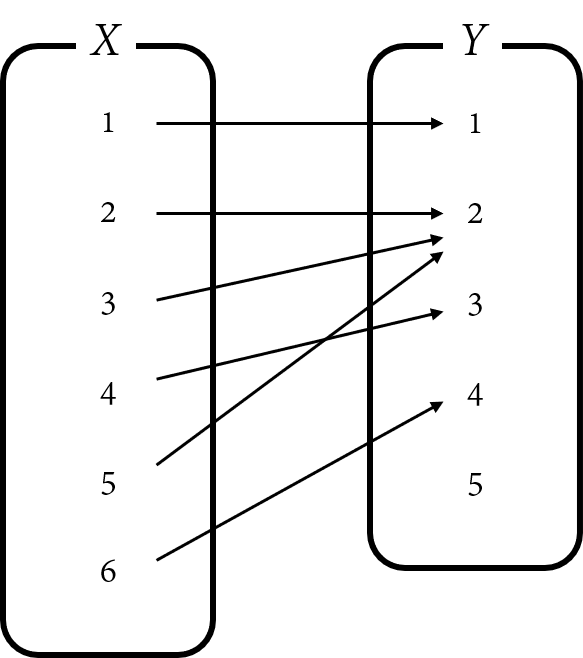
\includegraphics[width=0.24\textwidth]{graph_2-1}
\end{center}
의 그래프는
\begin{align*}
&\left\{\left(x,f(x)\right)\ba x=1,2,3,4,5,6\right\}\\
=&\{(1,f(1)),(2,f(2)),(3,f(3)),(4,f(4)),(5,f(5)),(6,f(6))\}\\
=&\{(1,1),(2,2),(3,2),(4,3),(5,2),(6,4)\}
\end{align*}
이다.
이것을 좌표평면 위에 나타내면 다음과 같다.
\begin{center}
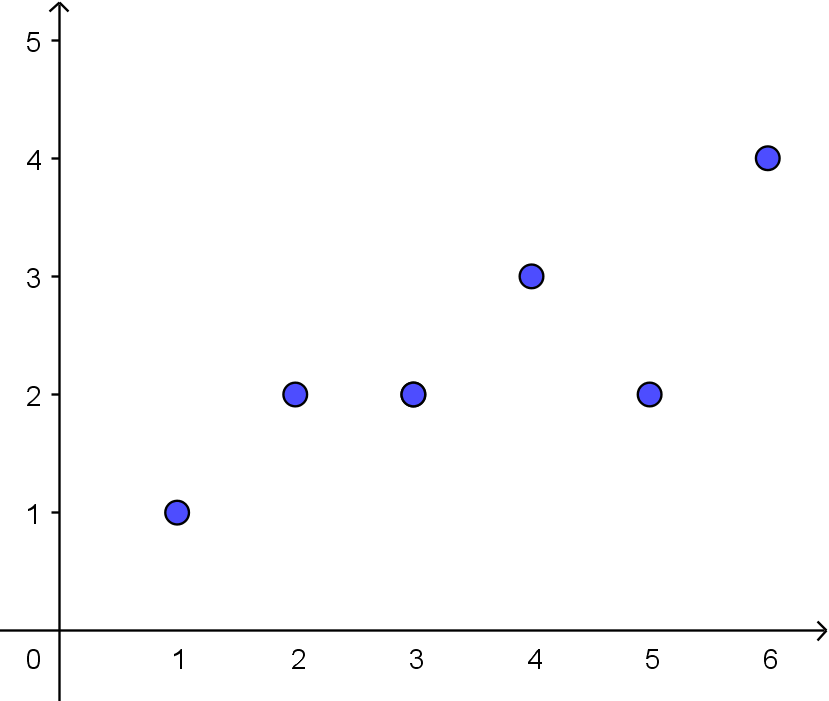
\includegraphics[width=0.3\textwidth]{graph_2-2}
\end{center}

%
\prob{}\label{graph3}
문제 \ref{function5})에서의 함수 \(f\)의 그래프를 그려라.

%
\exam{}\label{graph4}
함수 \(y=2x-4\)의 그래프를 그려라.
\begin{mdframed}
%\(f(x)=2x-4\)이고 
정의역은 실수 전체이므로 그래프는
\[\left\{\left(x,2x-4\right)\ba x\text{는 실수}\right\}\]
이다.
따라서 \((0,-4)\), \((1,-2)\), \((2,0)\), \((3,2)\) 등의 점들을 포함한다.
이것들을 모두 이으면 다음과 같은 직선이 된다.
\begin{center}
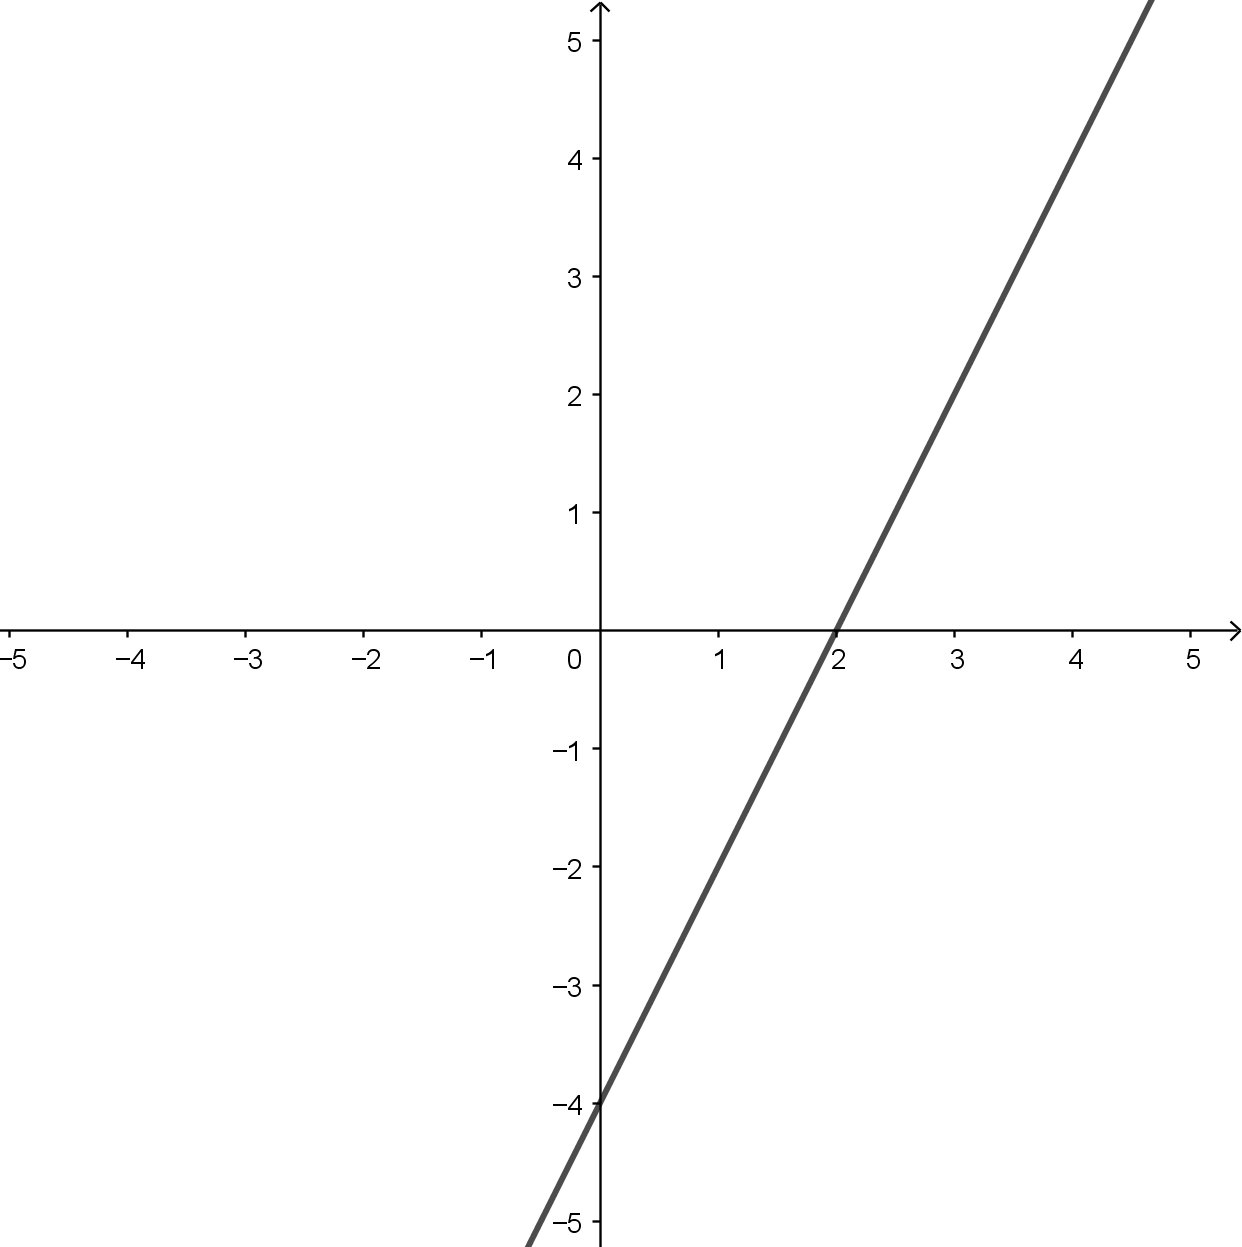
\includegraphics[width=0.4\textwidth]{graph_4}
\end{center}
이것은 평소에 그리던 \(y=2x-4\)의 그래프이다.
\end{mdframed}

%
\prob{다음 중 함수의 그래프인 것을 모두 골라라.}\label{graph5}
\begin{center}
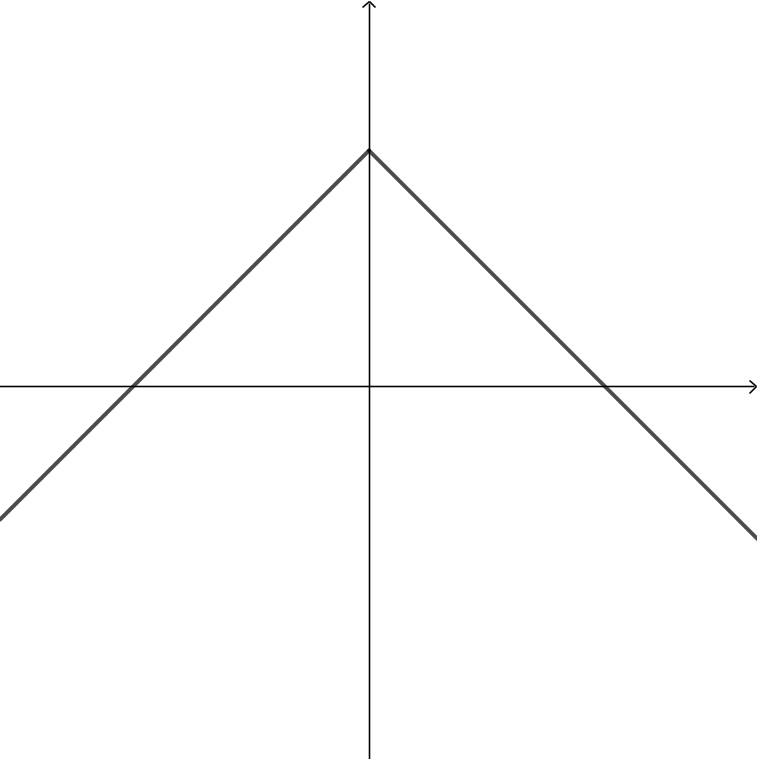
\includegraphics[width=0.22\textwidth]{graph_5-1}~~
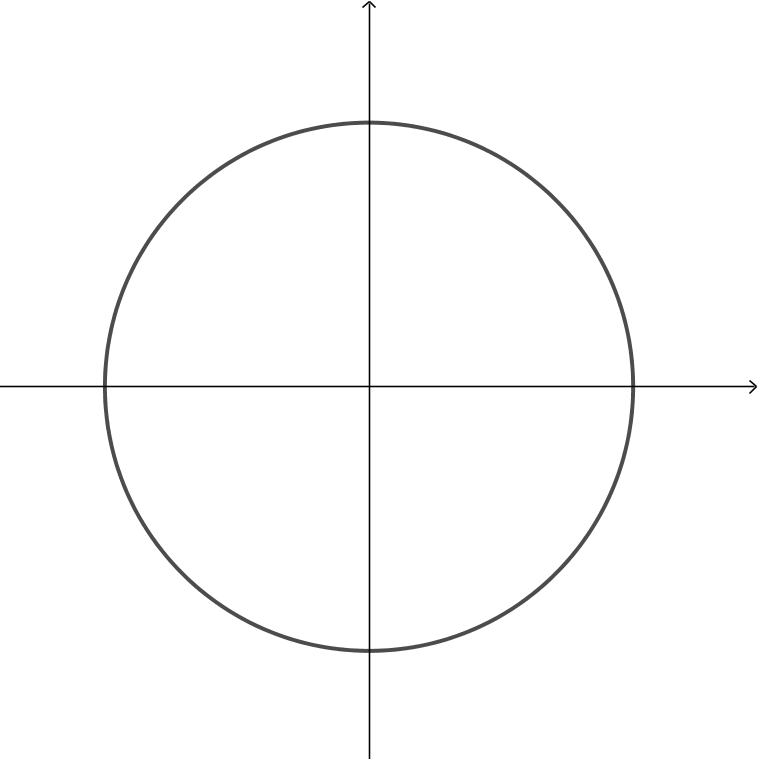
\includegraphics[width=0.22\textwidth]{graph_5-2}~~
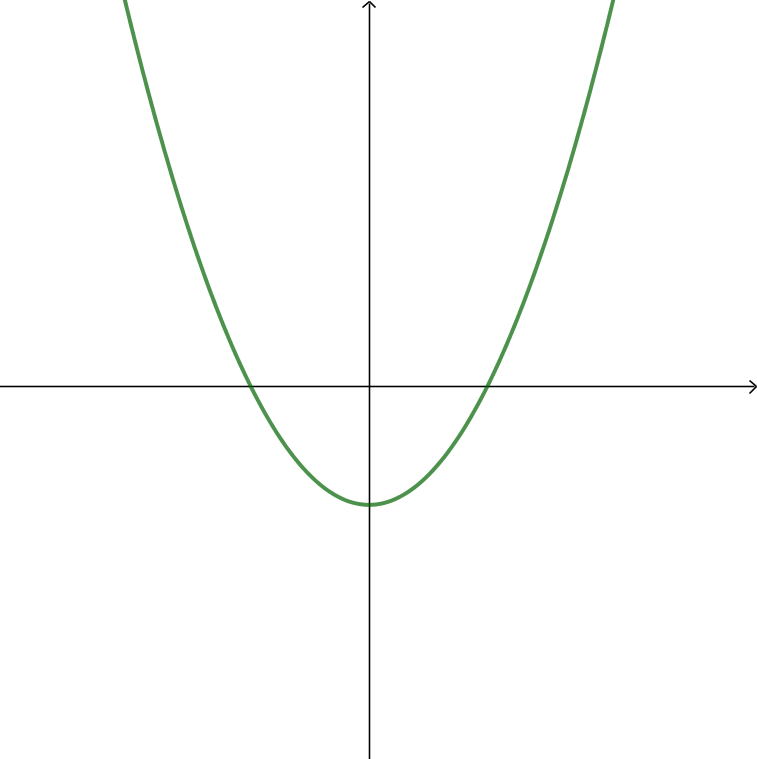
\includegraphics[width=0.22\textwidth]{graph_5-3}~~
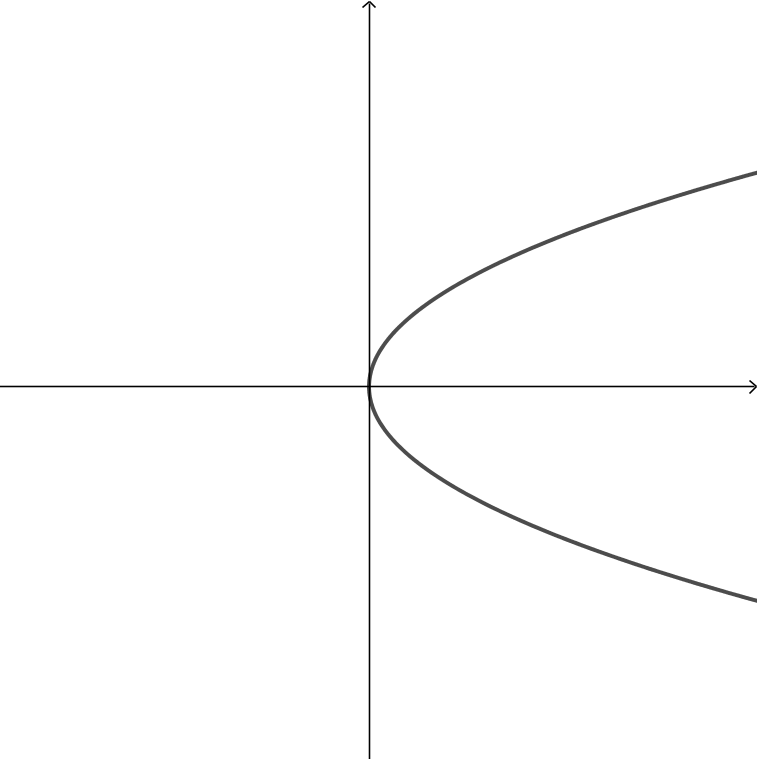
\includegraphics[width=0.22\textwidth]{graph_5-4}\\
(1)
\qquad\qquad\qquad\quad
(2)
\qquad\qquad\qquad\quad
(3)
\qquad\qquad\qquad\quad
(4)
\end{center}

%%
\section{여러가지 함수}
%%
%\exam{}\label{various1}
%어떤 대응이 함수이려면, 각각의 \(x\)값이 \(y\)값에 한 개씩 대응되어야 했었다.
%그래서 \(x\)값이 두 개 이상의 \(y\)값에 대응되는 (a)와 같은 경우는 함수라고 하지 않았다.
%이때 \(y\)에 대응되는 \(x\)값이 두 개 이상이어도 상관없었다.
%즉 (b)와 같은 경우도 함수라고 했었다.
%\(y\)에 대응되는 \(x\)값이 최대 한 개뿐인 (c)와 같은 함수를 \fbox{일대일함수}라고 한다.
%\begin{center}
%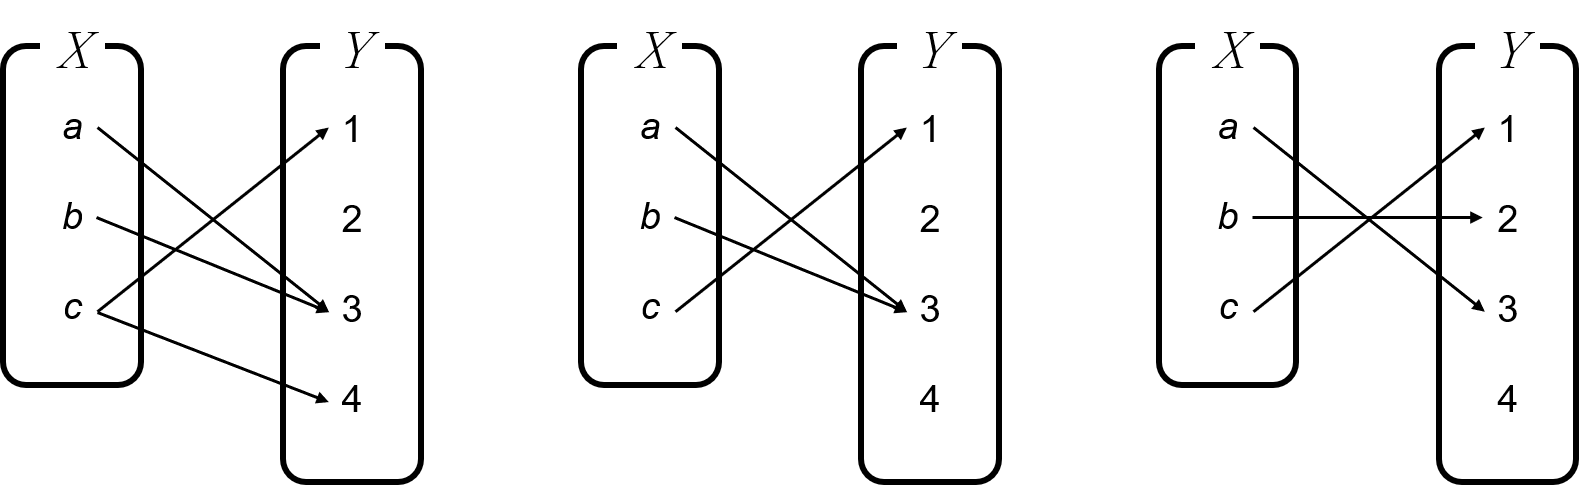
\includegraphics[width=0.99\textwidth]{various_1}\par
%\begin{tabu}{X[c]X[c]X[c]}
%(a)&(b)&(c)\\
%함수가 아니다. 	&함수이다. 			&함수이다.\\
%				&일대일함수가 아니다.	&일대일함수이다.\\
%				&					&일대일대응이 아니다.
%\end{tabu}
%\end{center}
%
%\begin{mdframed}
%%
%\defi{일대일함수}\label{various2}
%함수 \(f:X\to Y\)에서 \(x_1,x_2\in X\)일 때,
%\[x_1\neq x_2\Longrightarrow f(x_1)\neq f(x_2)\footnotemark\]
%이면 \(f\)를 일대일함수라고 부른다.
%\end{mdframed}
%\footnotetext{이것의 대우인
%\(f(x_1)=f(x_2)\Longrightarrow x_1=x_2\)
%를 만족시켜도 된다.
%}
%\newpage
%
%%
%\exam{}\label{various3}
%예시 \ref{various1})의 (c)의 경우, 모든 \(y\)값이 \(x\)값으로부터 대응되는 건 아니었다.
%\(1\), \(2\), \(3\)에 대응되는 \(x\)값이 하나씩 있었지만 \(4\)에는 대응되는 \(x\)값이 없었다.
%모든 \(y\)값이 \(x\)로부터 대응되는 (d)와 같은 경우를 \fbox{일대일대응}이라고 한다.
%\begin{center}
%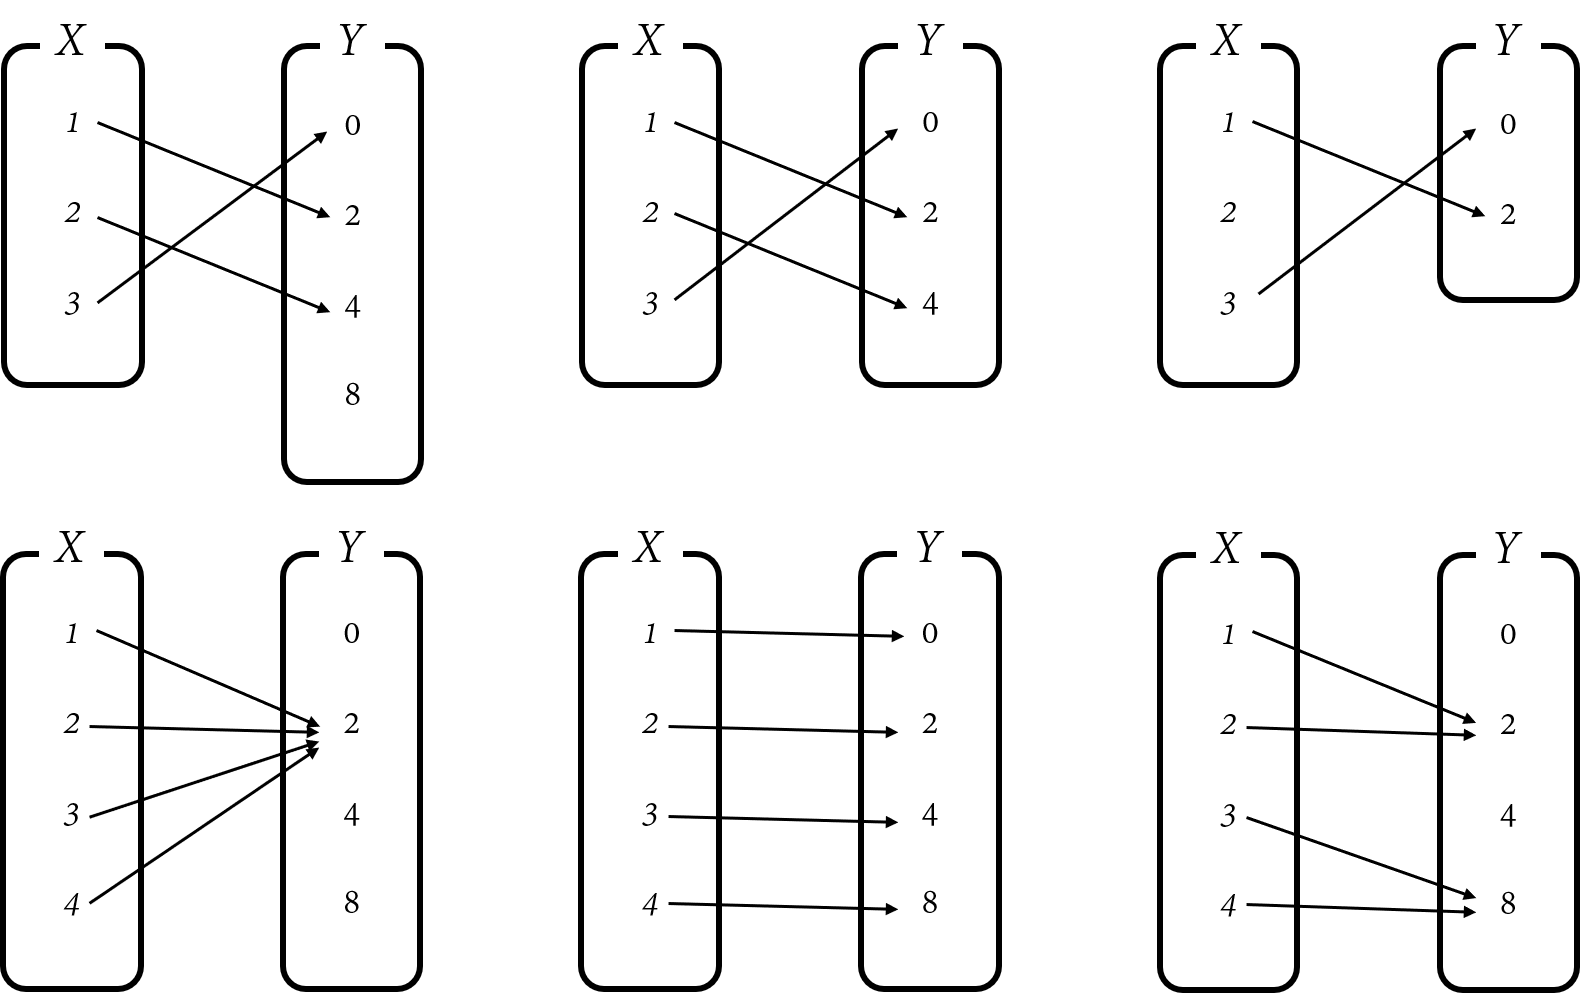
\includegraphics[width=0.25\textwidth]{various_3}\par
%(d)\\
%함수이다.\\
%일대일함수이다.\\
%일대일대응이다.
%\end{center}
%
%\begin{mdframed}
%%
%\defi{일대일대응}\label{various4}
%함수 \(f:X\to Y\)가 다음 두 조건을 만족시키면 일대일대응이라고 부른다.
%\begin{enumerate}[label=\roman*)]
%\item
%\(f\)가 일대일함수이다.
%\item
%공역과 치역이 같다.
%\end{enumerate}
%\end{mdframed}

어떤 대응이 함수이려면, 각각의 \(x\)값이 \(y\)값에 한 개씩 대응되어야 했었다.
그래서 \(x\)값이 두 개 이상의 \(y\)값에 대응되는 (가)와 같은 경우는 함수라고 하지 않았다.
이때 \(y\)에 대응되는 \(x\)값이 두 개 이상이어도 상관없었다.
즉 (나)와 같은 경우도 함수라고 했었다.
\(y\)에 대응되는 \(x\)값이 최대 한 개뿐인 (다)와 같은 함수를 \fbox{일대일함수}라고 한다.
\begin{mdframed}
%
\defi{일대일함수}\label{various1}
함수 \(f:X\to Y\)에서 \(x_1,x_2\in X\)일 때,
\[x_1\neq x_2\Longrightarrow f(x_1)\neq f(x_2)\footnotemark\]
이면 \(f\)를 일대일함수라고 부른다.
\end{mdframed}
\footnotetext{이것의 대우인
\(f(x_1)=f(x_2)\Longrightarrow x_1=x_2\)
를 만족시켜도 된다.
}

\bigskip\bigskip
(다)의 경우, 모든 \(y\)값이 어떤 \(x\)값으로부터 대응되는 건 아니었다.
\(1\), \(2\), \(3\)에 대응되는 \(x\)값은 하나씩 있었지만 \(4\)에 대응되는 \(x\)값은 없었다.
모든 \(y\)값이 \(x\)로부터 대응되는 (라)와 같은 경우를 \fbox{일대일대응}이라고 한다.
\begin{mdframed}
%
\defi{일대일대응}\label{various2}
함수 \(f:X\to Y\)가 다음 두 조건을 만족시키면 일대일대응이라고 부른다.
\begin{enumerate}[label=\roman*)]
\item
\(f\)가 일대일함수이다.
\item
공역과 치역이 같다.
\end{enumerate}
\end{mdframed}
%이상을 정리하면
%
%\begin{quote}
%함수 : 모든 \(x\)가 단 하나의 \(y\)에  대응된다.\\
%일대일함수 : 함수이면서, \(y\)에 대응되는 \(x\)가 한 개 이하이다.\\
%일대일대응 : 함수이면서, \(y\)에 대응되는 \(x\)가 한 개이다.
%\end{quote}
\begin{center}
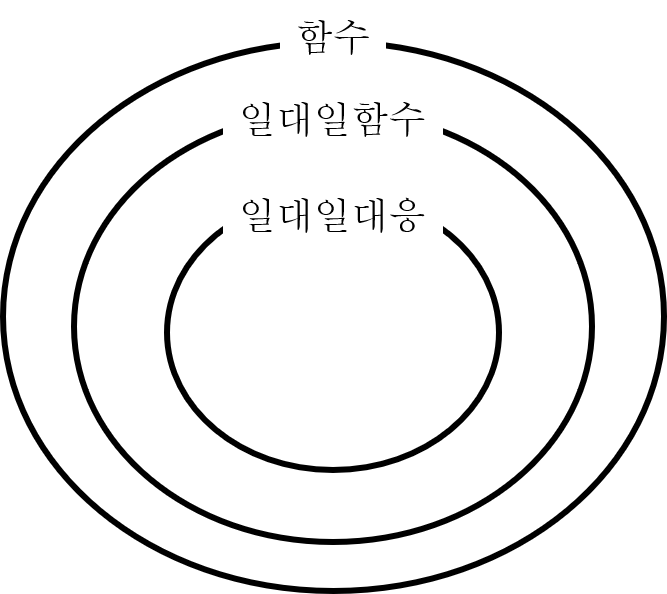
\includegraphics[width=0.3\textwidth]{various_2}
\end{center}



\newpage
\begin{center}
\begin{tabu}{X[c]X[c]X[c]X[c]}
(가)				&(나)				&(다)				&(라)\\
\end{tabu}
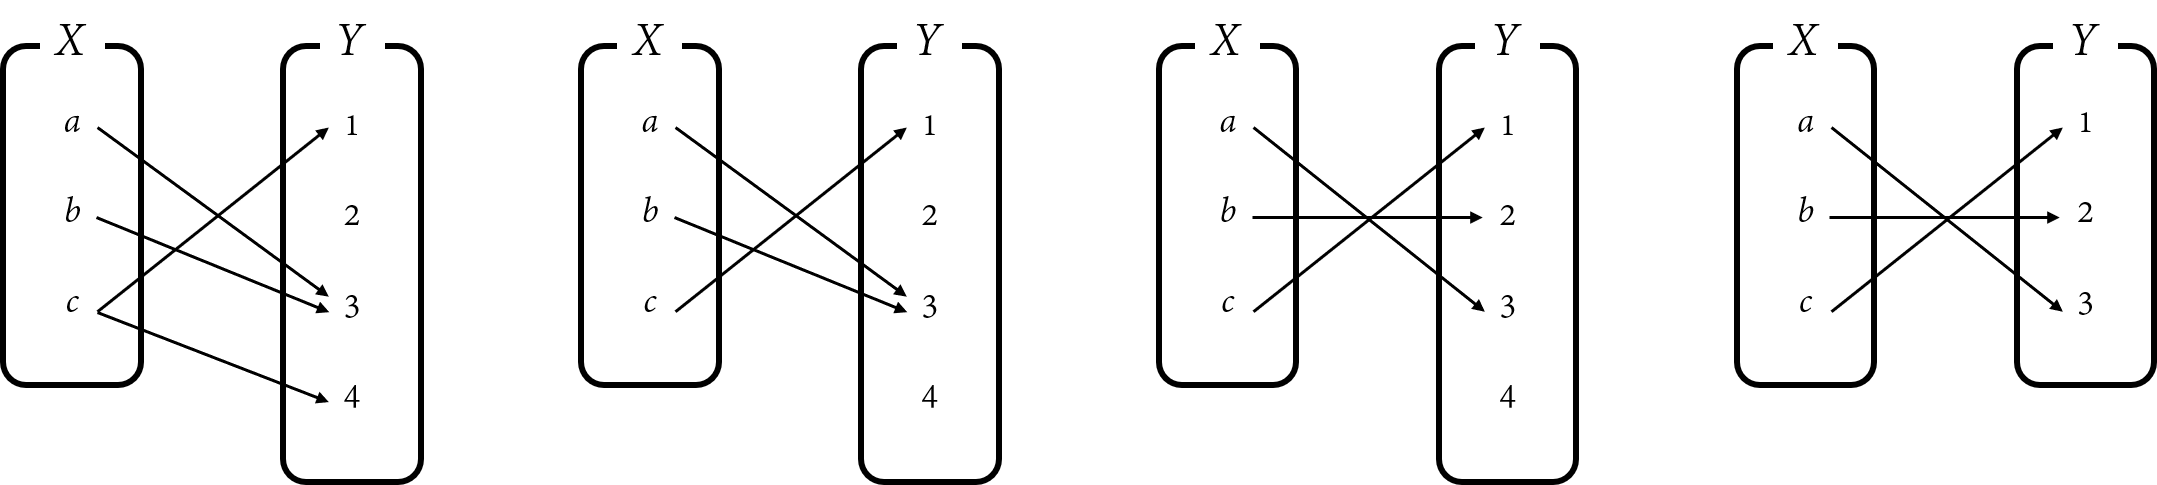
\includegraphics[width=0.9\textwidth]{various_0}\par
\begin{tabu}{>{\scriptsize}X[c]>{\scriptsize}X[c]>{\scriptsize}X[c]>{\scriptsize}X[c]}
%(a)				&(b)					&(c)					&(d)\\
함수가 아니다. 	&함수이다. 			&함수이다.			&함수이다.\\
				&일대일함수가 아니다.	&일대일함수이다.		&일대일함수이다.\\
				&					&일대일대응이 아니다.	&일대일대응이다.
\end{tabu}
\end{center}

%\begin{center}
%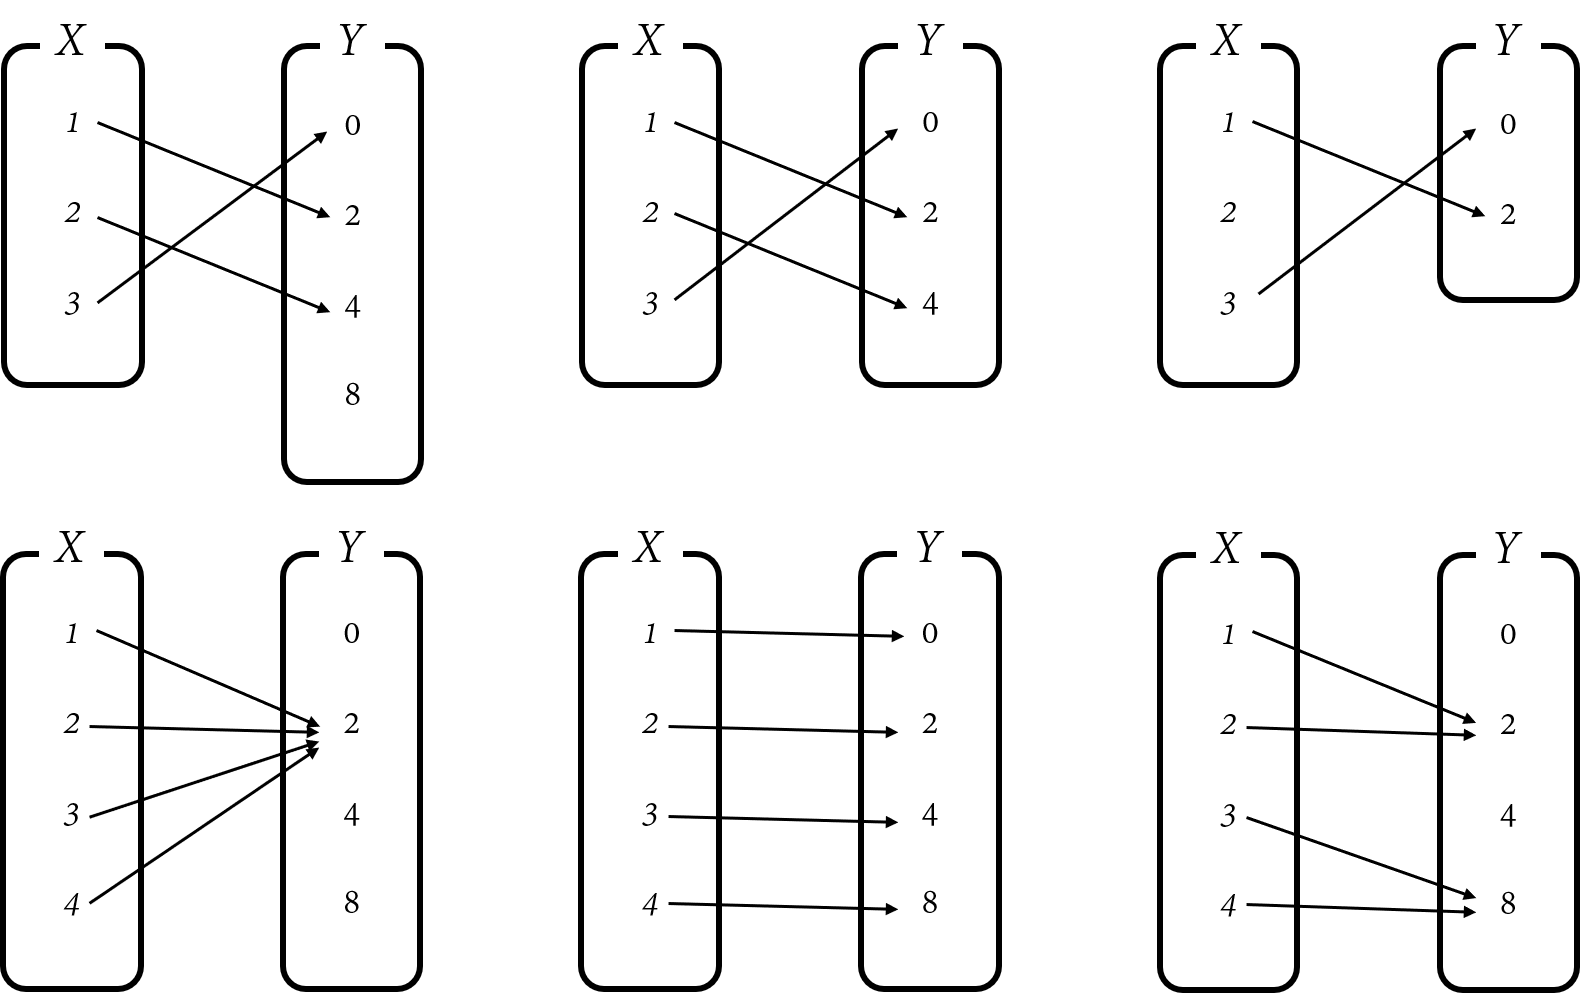
\includegraphics[width=0.25\textwidth]{various_3}\par
%(d)\\
%함수이다.\\
%일대일함수이다.\\
%일대일대응이다.
%\end{center}

%
\prob{}\label{various3}
다음 여섯 개의 대응 중 함수의 개수를 \(a\), 일대일함수의 개수를 \(b\),  일대일대응의 개수를 \(c\)라고 할 때, \(a\), \(b\), \(c\)의 값을 각각 구하여라.
\begin{center}
(1)\hspace{100pt}(2)\hspace{100pt}(3)\\
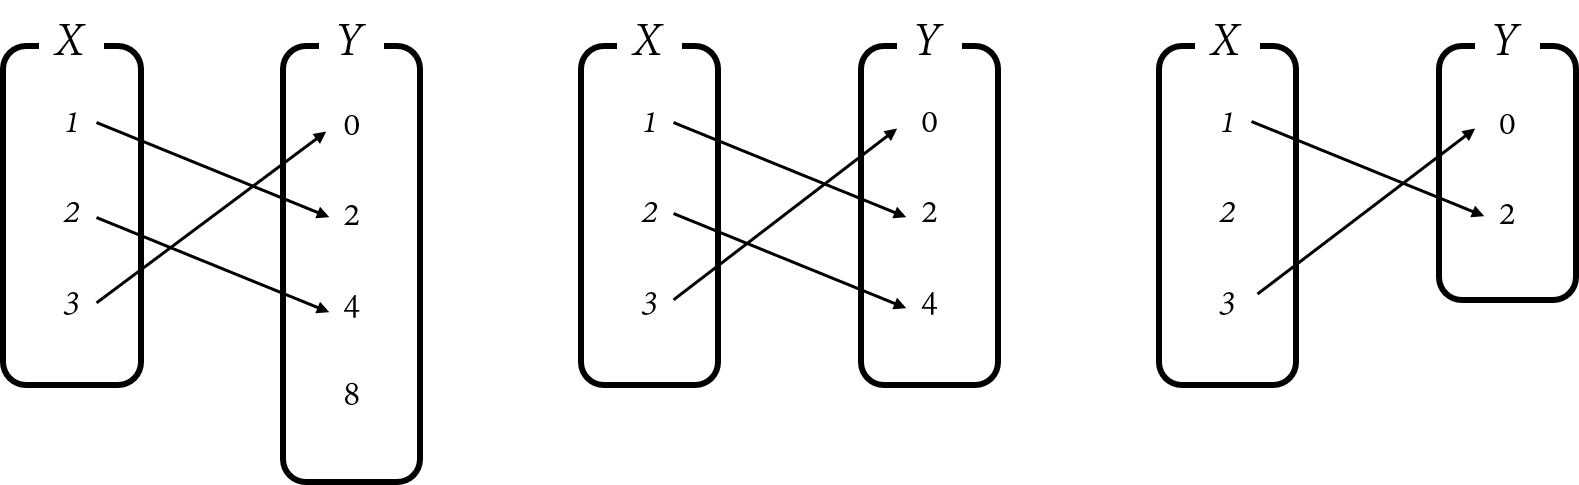
\includegraphics[width=0.9\textwidth]{various_3-1}\\[10pt]
(4)\hspace{100pt}(5)\hspace{100pt}(6)\\
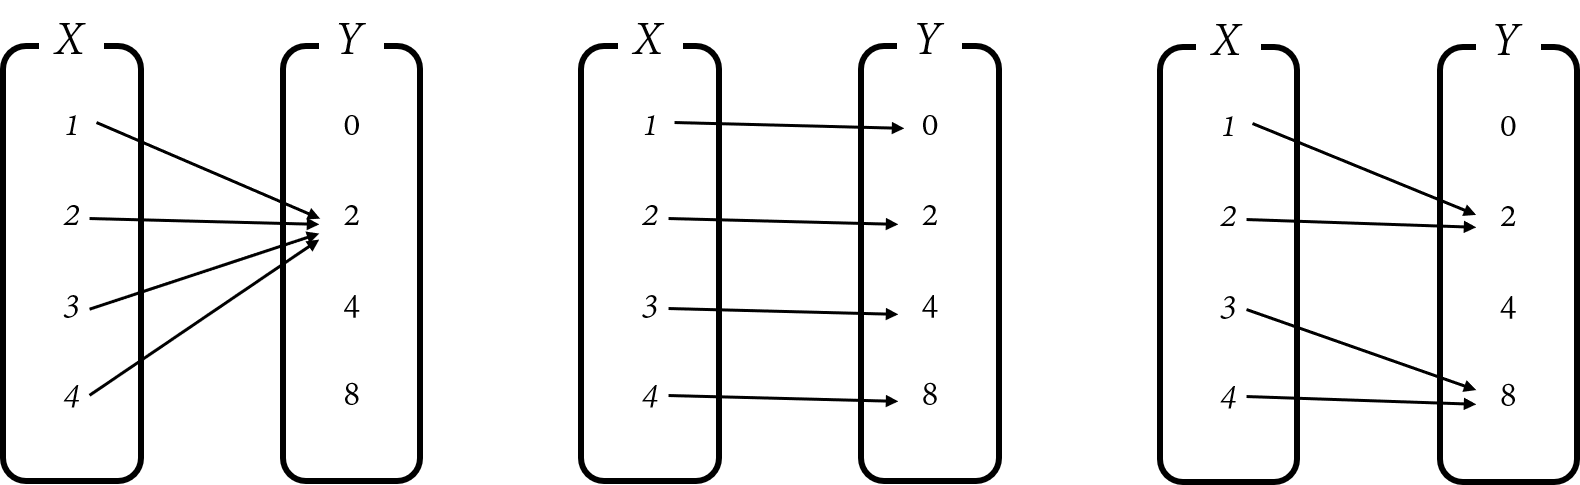
\includegraphics[width=0.9\textwidth]{various_3-2}
\end{center}

\newpage
%
\exam{다음 함수들의 종류를 조사하여라.}
\begin{enumerate*}[itemjoin={\tabto{0.5\textwidth}}]\label{various4}
\item
\(y=2x-4\)
\item
\(y=x^2\)
\end{enumerate*}
\begin{mdframed}[frametitle=방법1]
두 함수의 정의역과 공역은 모두 실수전체의 집합이다.
%하지만 
모든 실수의 대응관계를 다 나타낸다는 것은 불가능한 일이므로 몇 개의 정수에 대해서만 대응관계를 나타내면 다음과 같다.
\begin{center}
(1)\hspace{120pt}(2)\\
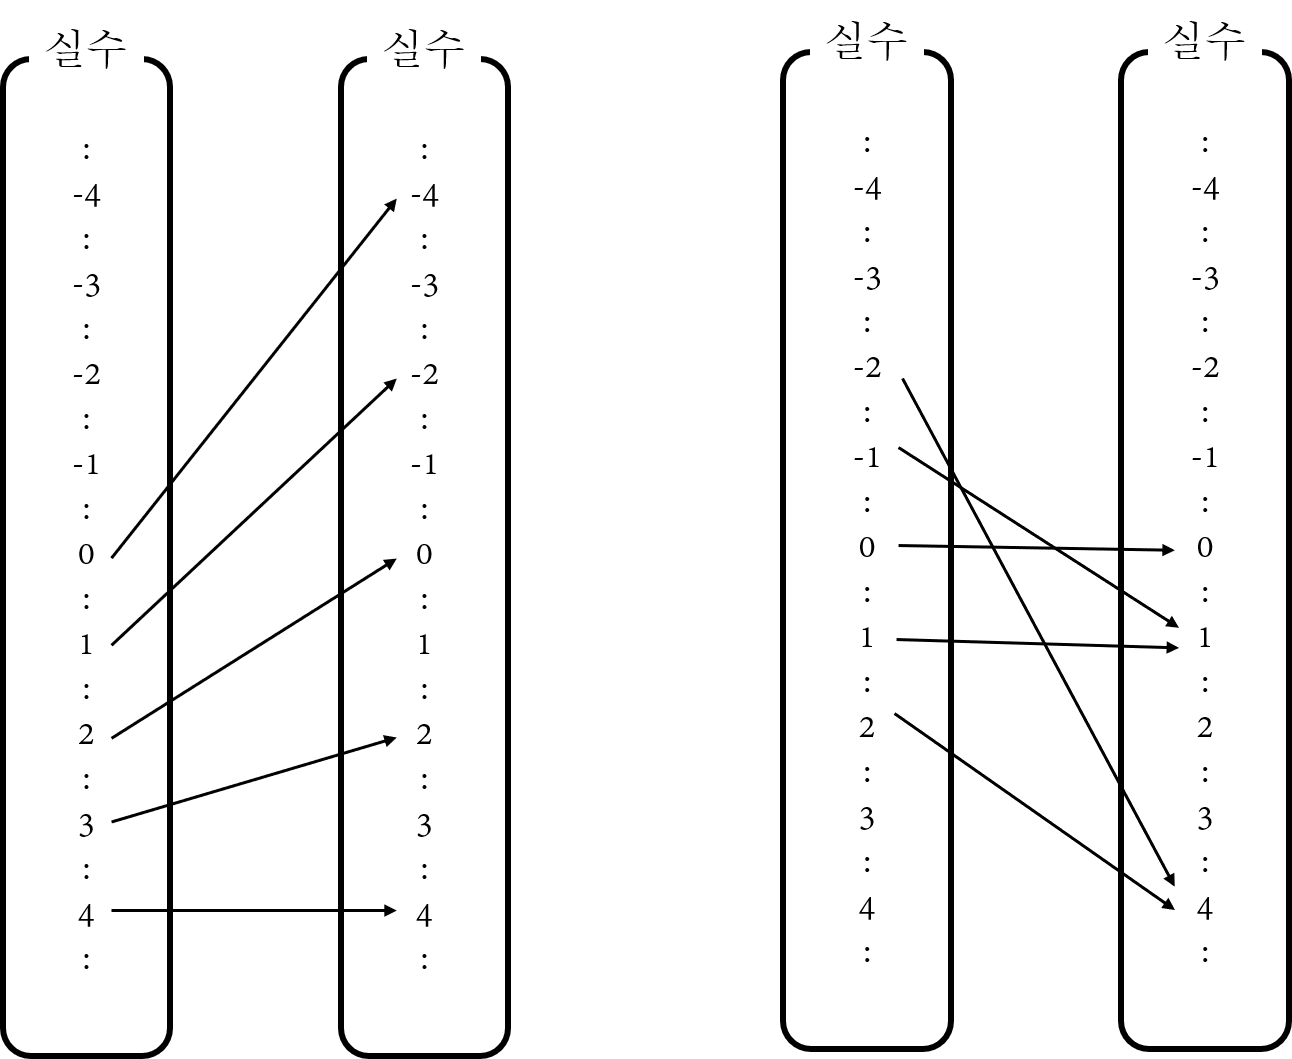
\includegraphics[width=0.7\textwidth]{various_4-1}
\end{center}

(1) 두 개 이상의 \(x\)값이 하나의 \(y\)값에 대응되지 않는다.
따라서 일대일함수이다.\footnotemark[1]
%또한 치역이 실수 전체의 집합이다.
%그림에서만 보면 치역에 속하는 원소가 \(-4\), \(-2\), \(0\), \(2\), \(4\) 뿐인 것처럼 보이기 때문에 \(-3\)이 치역에서 제외된 것처럼 보이지만 \(-3\)도 치역의 원소이다.
%\(f\left(\frac12\right)=-3\)이기 떄문이다.
정의역과 공역이 무한집합이라 화살표로 다 표시할 수는 없지만, 모든 실수들은 함숫값이다.
따라서 치역은 실수 전체의 집합이고 이 함수는 일대일대응이다.

(2) 두 개의 \(x\)값이 하나의 \(y\)값에 대응되는 경우가 있다.
예를 들어 \(-2\)와 \(2\)는 모두 \(4\)로 대응된다.
따라서 일대일함수가 아니다.\footnotemark[2]
\end{mdframed}
\footnotetext[1]{다음과 같이 해도 된다 ;
\par\noindent
\(f(x_1)=f(x_2)\)이면, \(2x_1-4=2x_2-4\)이고 \(2x_1=2x_2\)이다.
따라서 \(x_1=x_2\)이다.
[정리 \ref{various1})]\\
%\begin{align*}
%2x_1-4=2x_2-4\\
%2x_1=2x_2\\
%x_1=x_2
%\end{align*}
%이다.
%정리 \ref{various1})에 의해 이 함수는 일대일함수이다.
}
\footnotetext[2]{\(x_1=-2\), \(x_2=2\)는 명제 \(x_1\neq x_2\longrightarrow f(x_1)\neq f(x_2)\)의 반례가 된다.}

\newpage
\begin{mdframed}[frametitle=방법2,nobreak=false]
두 함수의 그래프를 그리면 다음과 같다.
\begin{center}
(1)\hspace{120pt}(2)\\[10pt]
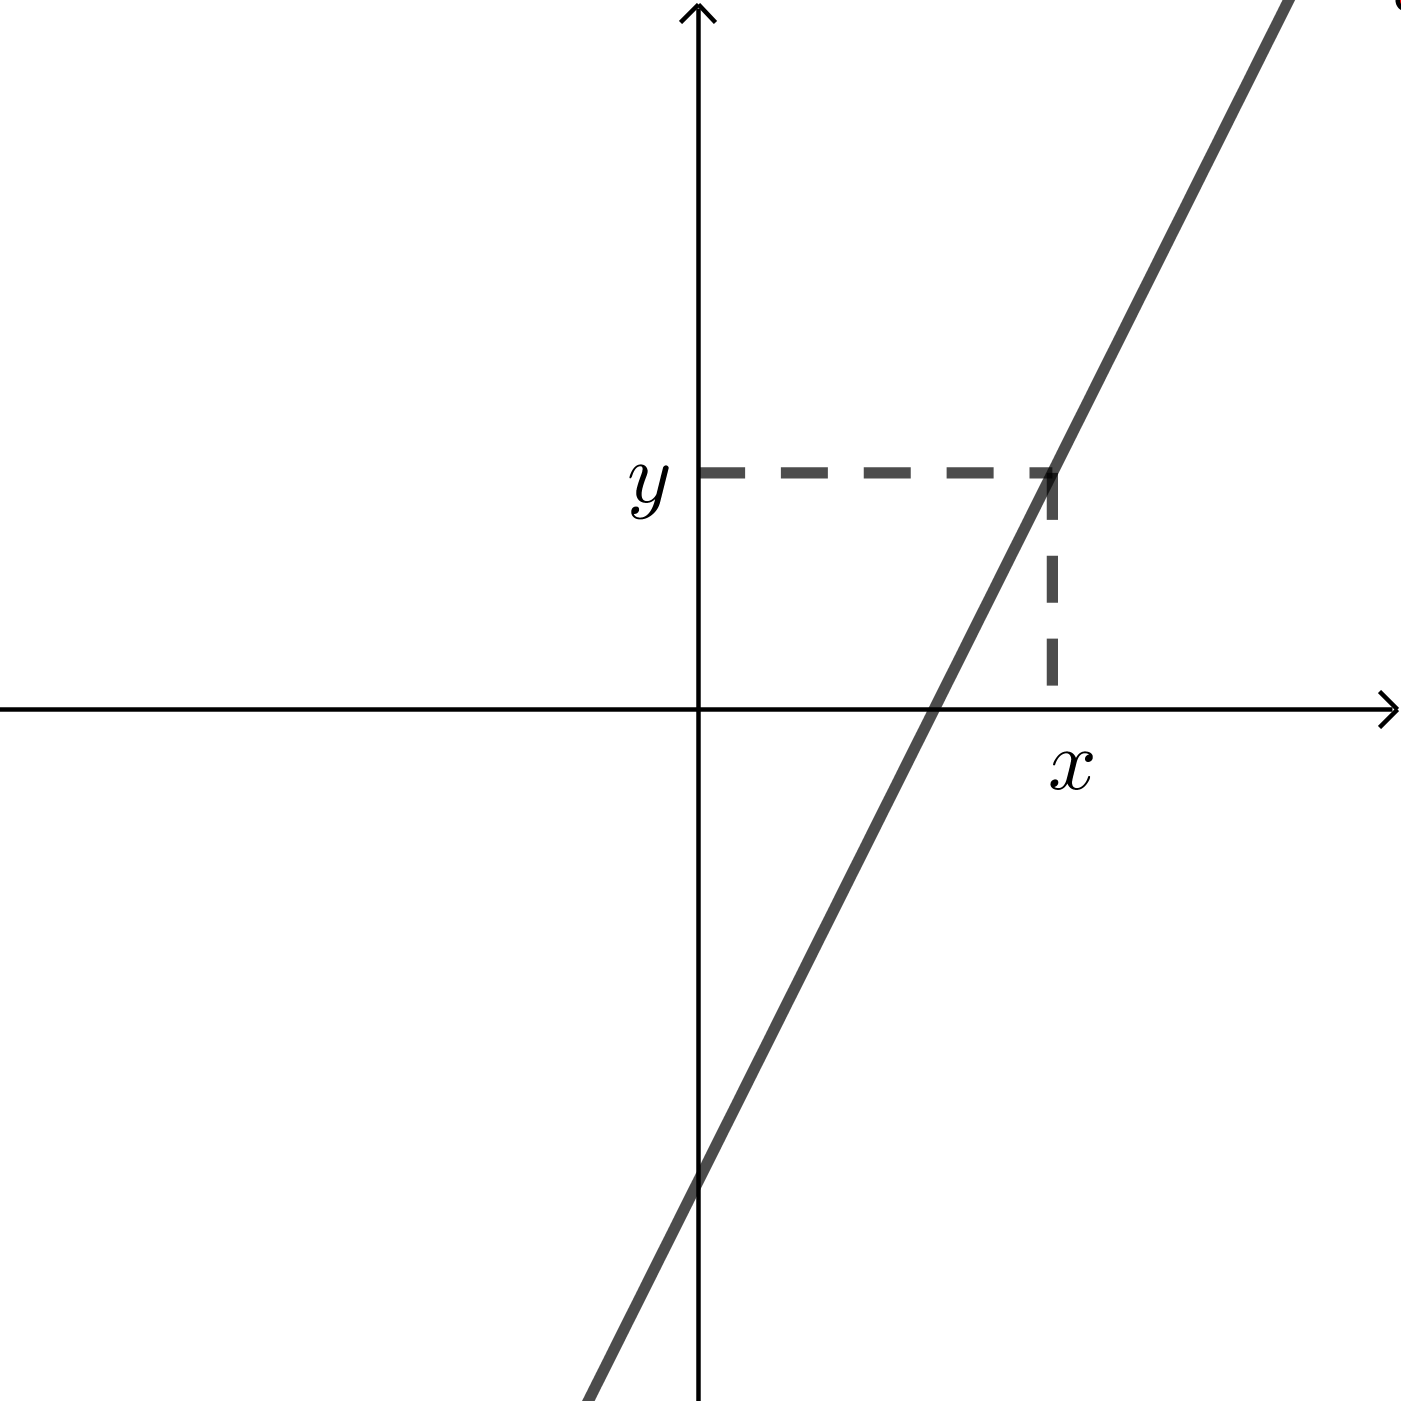
\includegraphics[width=0.3\textwidth]{various_4-2}\qquad\qquad
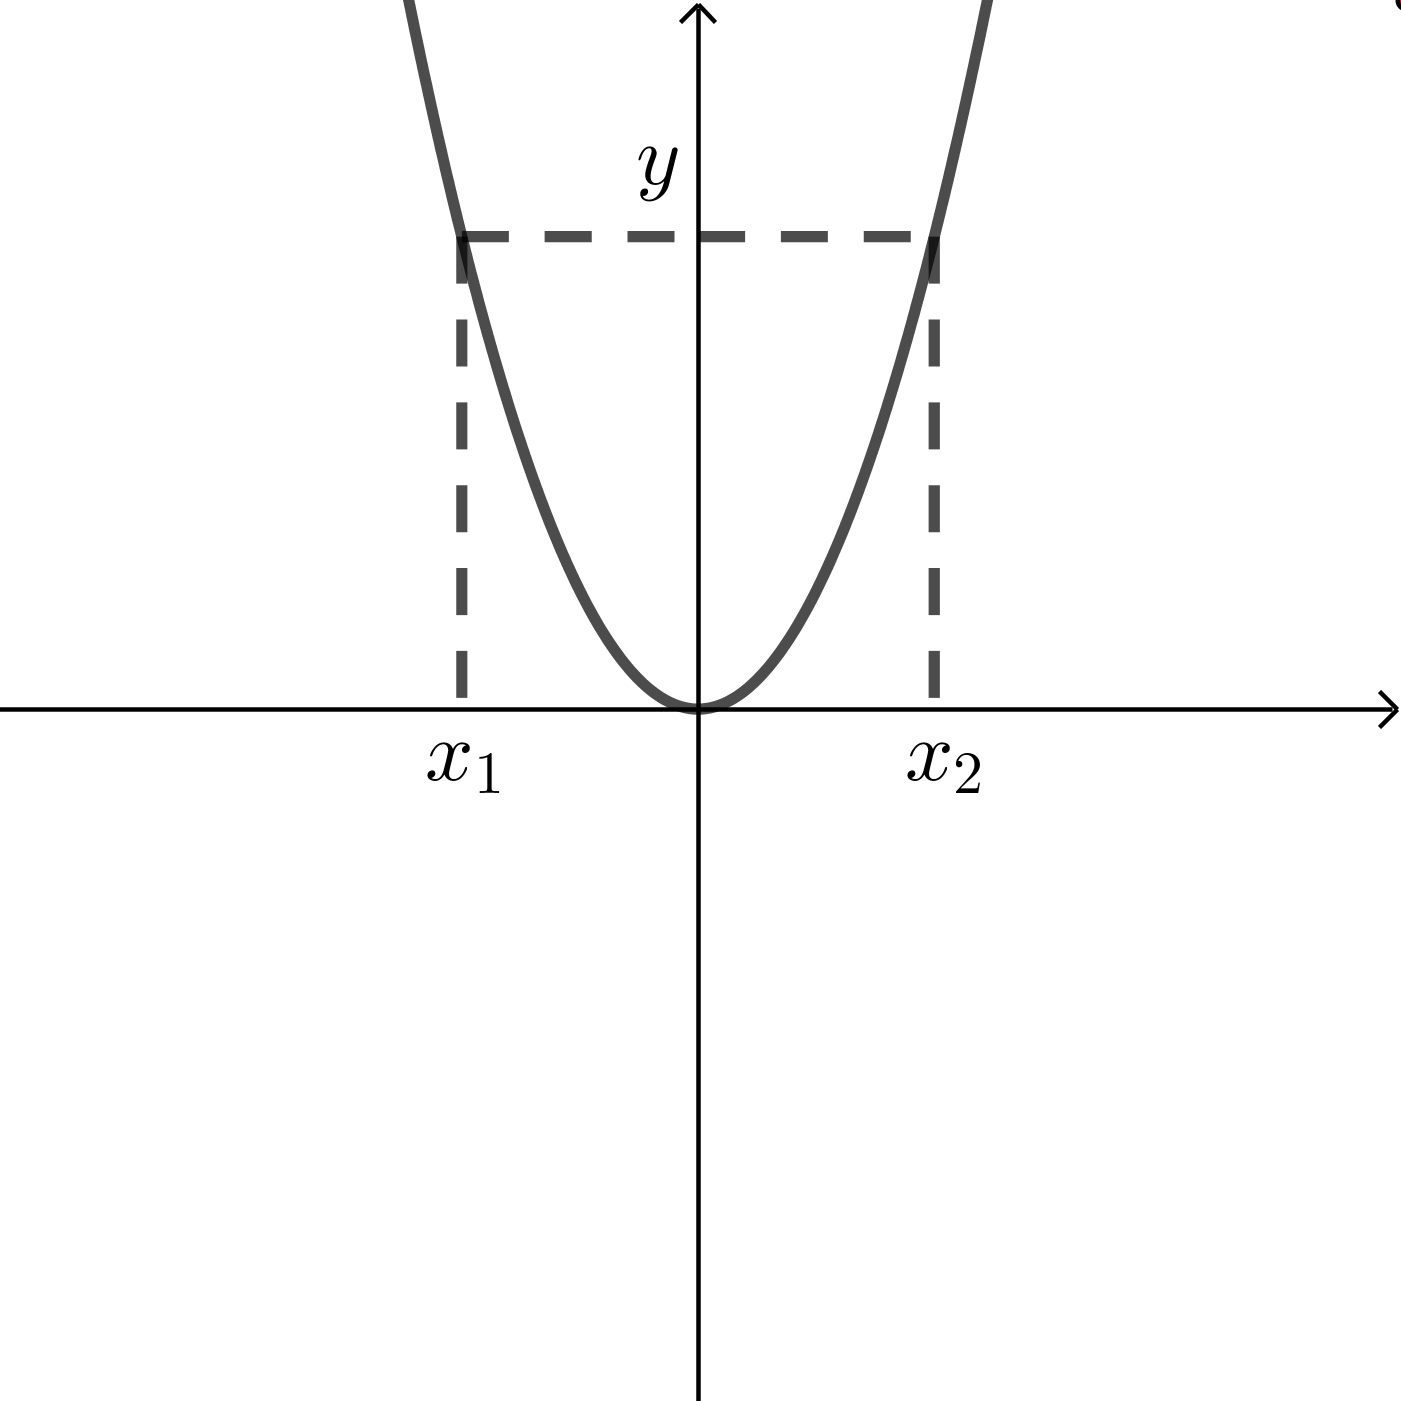
\includegraphics[width=0.3\textwidth]{various_4-3}
\end{center}

(1) %\(x\)값이 하나 주어지면 그에 대응되는 \(y\)값이 항상 한 개 존재한다.
%따라서 함수이다.
%또한, 
두 개 이상의 \(x\)값이 하나의 \(y\)값에 대응되는 일이 없다.
따라서 일대일함수이다.
%마지막으로,
또한
치역은 실수 전체의 집합이어서 공역과 같다.
따라서 일대일대응이다.

(2)% \(x\)값이 하나 주어지면 그에 대응되는 \(y\)값이 항상 한 개 존재한다.
%따라서 함수이다.
%하지만, 그림에서 보듯 
양수 \(y\)에 대해, \(y\)로 대응되는 \(x\)값은 두 개 존재한다.
따라서 일대일함수가 아니다.
\end{mdframed}
\ans{\parbox[t]{.45\textwidth}{
(1) 일대일대응이다.\\
(2) 일대일함수가 아닌 함수이다.}}
%\ans{\pbox{
%(1) 일대일대응이다.
%(2) 일대일함수가 아닌 함수이다.}}

%
\prob{}\label{various5}
다음 네 개의 그래프가 나타내는 대응에 대하여,
함수의 개수를 \(a\), 일대일함수의 개수를 \(b\), 일대일대응의 개수를 \(c\)라고 할 때 \(a\), \(b\), \(c\)의 값을 각각 구하여라.
\begin{center}
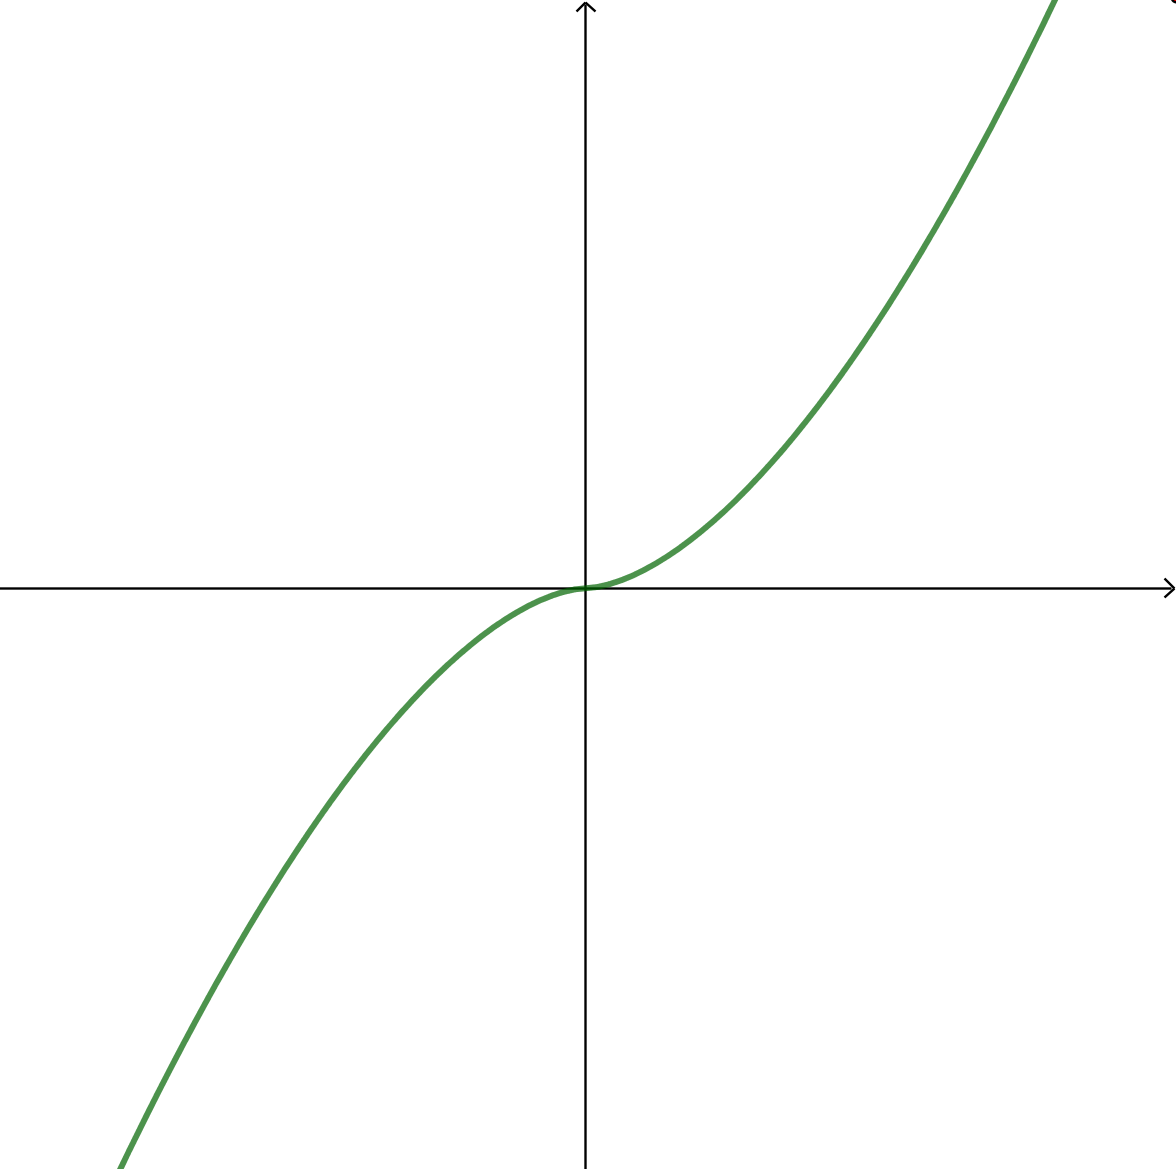
\includegraphics[width=0.22\textwidth]{various_5-1}~~
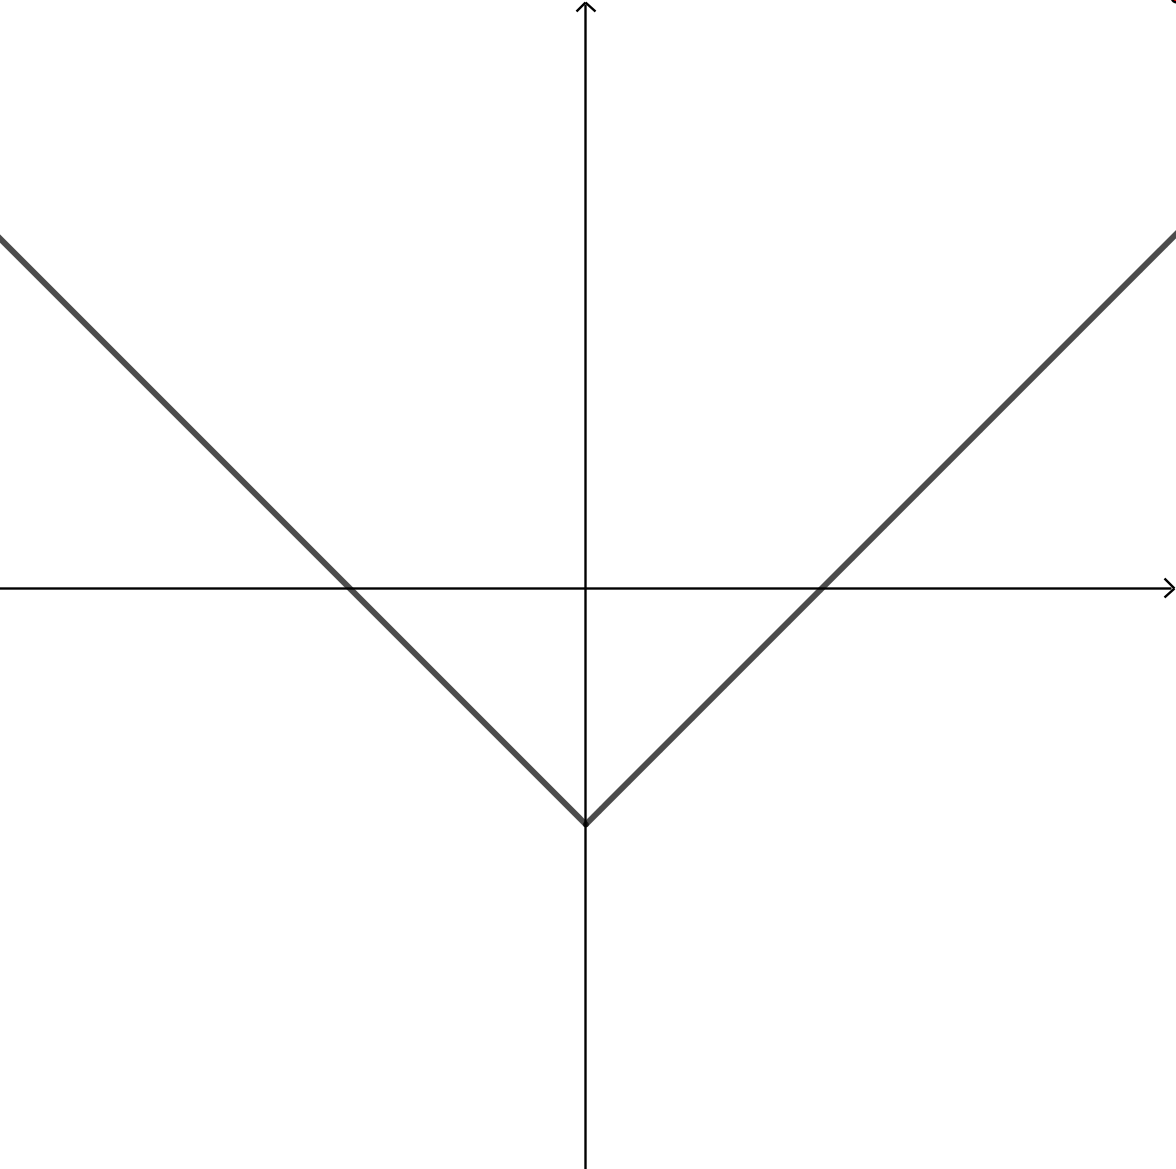
\includegraphics[width=0.22\textwidth]{various_5-2}~~
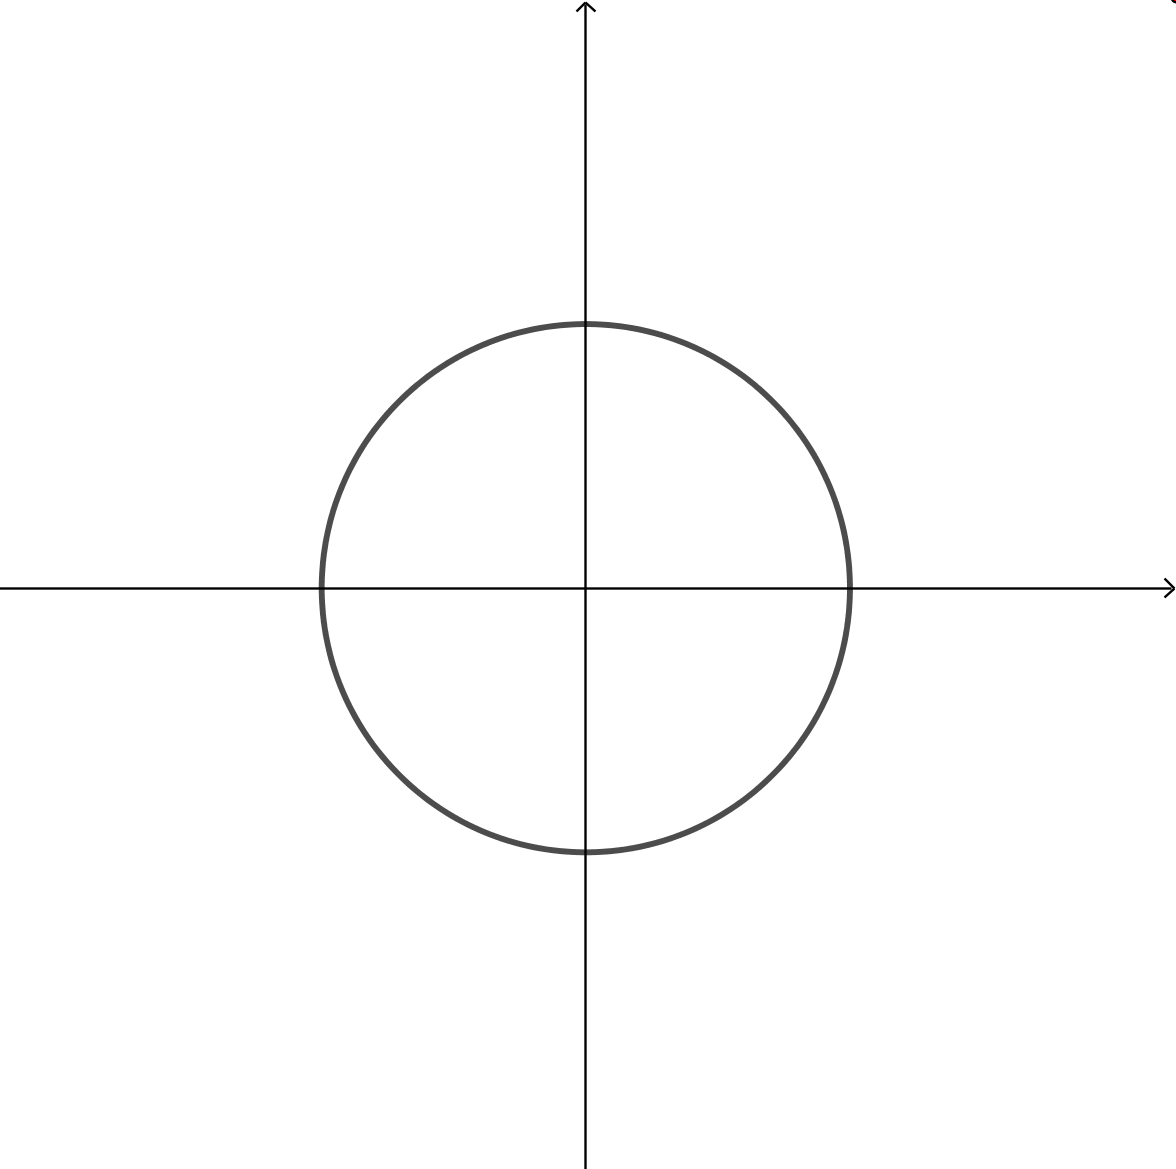
\includegraphics[width=0.22\textwidth]{various_5-3}~~
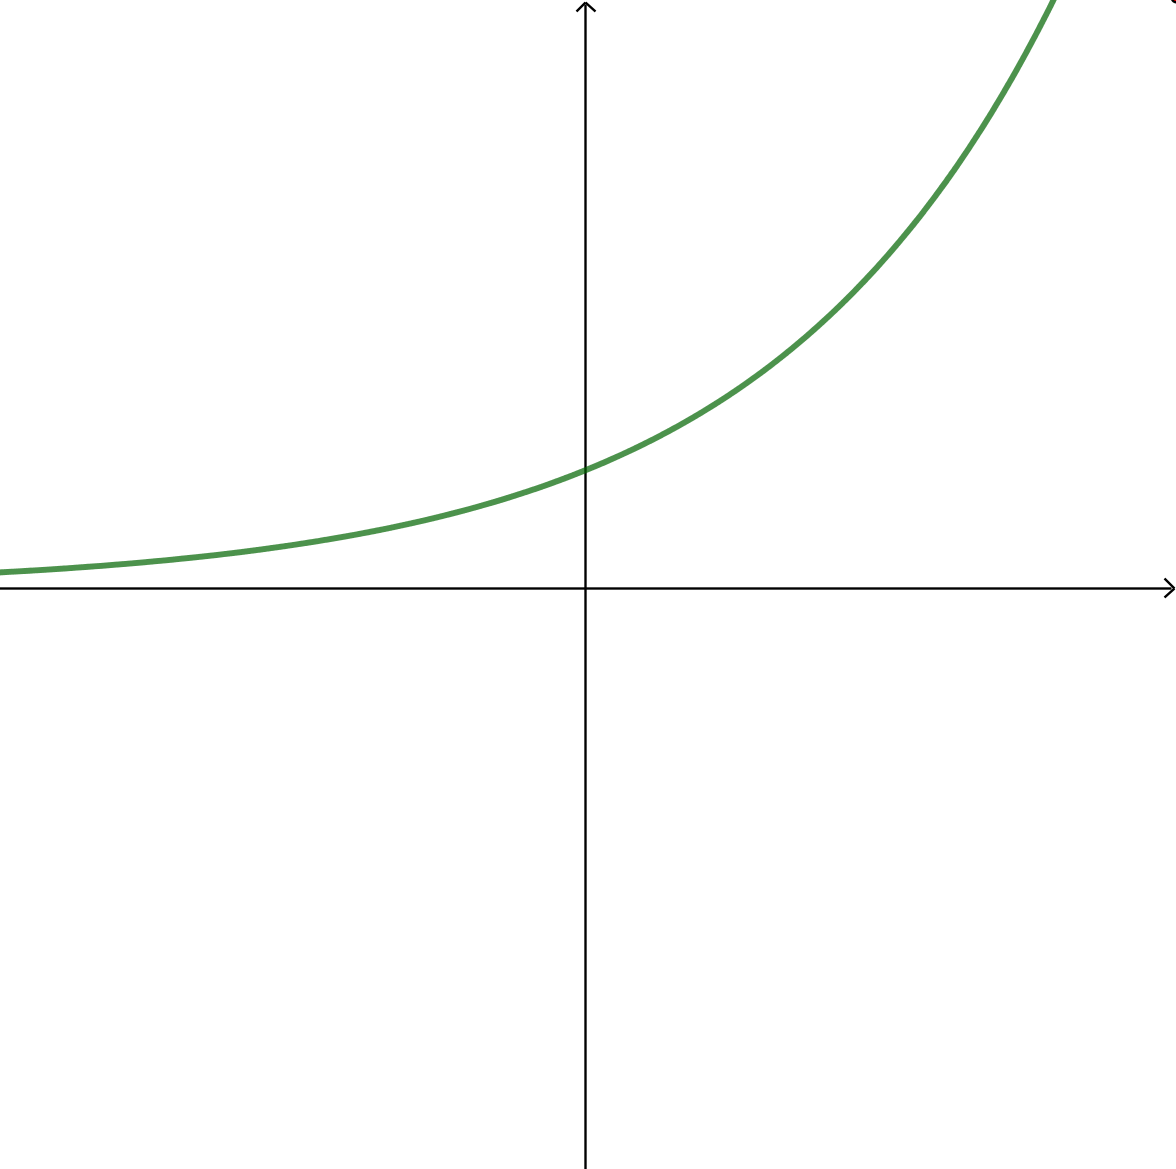
\includegraphics[width=0.22\textwidth]{various_5-4}\\
(1)
\qquad\qquad\qquad\quad
(2)
\qquad\qquad\qquad\quad
(3)
\qquad\qquad\qquad\quad
(4)
\end{center}

\begin{mdframed}
%
\defi{항등함수}\label{various6}
정의역과 공역이 같은 함수 \(f:X\to X\)가
\[f(x)=x\]
로 정의되면 이 함수를 \fbox{항등함수}라고 부른다.
\end{mdframed}
항등함수는 기호로 \(I\)라고 쓰기도 한다.
또한, 정의역과 공역이 \(X\)임을 강조하기 위해 \(I_X\)라고 쓰기도 한다.

\begin{mdframed}
%
\defi{상수함수}\label{various7}
함수 \(f:X\to Y\)가
\[f(x)=c\quad(c\text{는 상수})\]
로 정의되면 이 함수를 \fbox{상수함수}라고 부른다.
\end{mdframed}

%
\exam{두 집합 \(X=\{1,2,3\}\), \(Y=\{2,4\}\)에 대하여}\label{various8}
두 함수 \(f:X\to X\)와 \(g:X\to Y\)가
%\(f=I=I_X\)이다.
%따라서 \(I(1)=1\), \(I(2)=2\), \(I(3)=3\)이다.
%또 \(I_X(1)=1\), \(I_X(2)=2\), \(I_X(3)=3\)이다.
\begin{center}
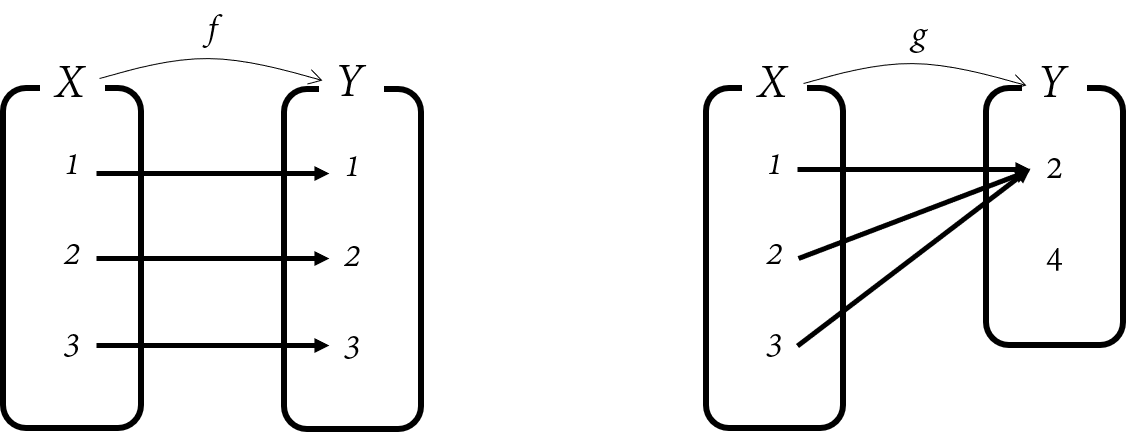
\includegraphics[width=0.5\textwidth]{various_8}
\end{center}
%위의 그림과 같이 정의되면
와 같이 주어지면
\begin{align*}
f(1)&=1,\qquad g(1)=2\\
f(2)&=2,\qquad g(2)=2\\
f(3)&=3,\qquad g(3)=2
\end{align*}
이므로 함수 \(f\)는 항등함수이고\footnotemark\:\:함수 \(g\)는 상수함수이다.
\footnotetext{\(f=I=I_X\)이다.
따라서
\parbox[t]{40pt}{\(I(1)=1\),\\\(I(2)=2\)\\\(I(3)=3\)}
\parbox[t]{40pt}{\(I_X(1)=1\)\\\(I_X(2)=2\)\\\(I_X(3)=3\)}
이라고 쓸 수 있다.}

%
\prob{\normalsize{예시 \ref{various8})에서}}
\begin{itemize}\label{various9}
\item
\(f\)는 (일대일함수이다 / 일대일함수가 아니다)
\item
\(f\)는 (일대일대응이다 / 일대일대응이 아니다)
\item
\(g\)는 (일대일함수이다 / 일대일함수가 아니다)
\item
\(g\)는 (일대일대응이다 / 일대일대응이 아니다)
\end{itemize}

%
\prob{다음 중에서 항등함수와 상수함수의 그래프를 각각 찾으시오.}\label{various10}
\begin{center}
(1)\hspace{100pt}(2)\hspace{100pt}(3)\\
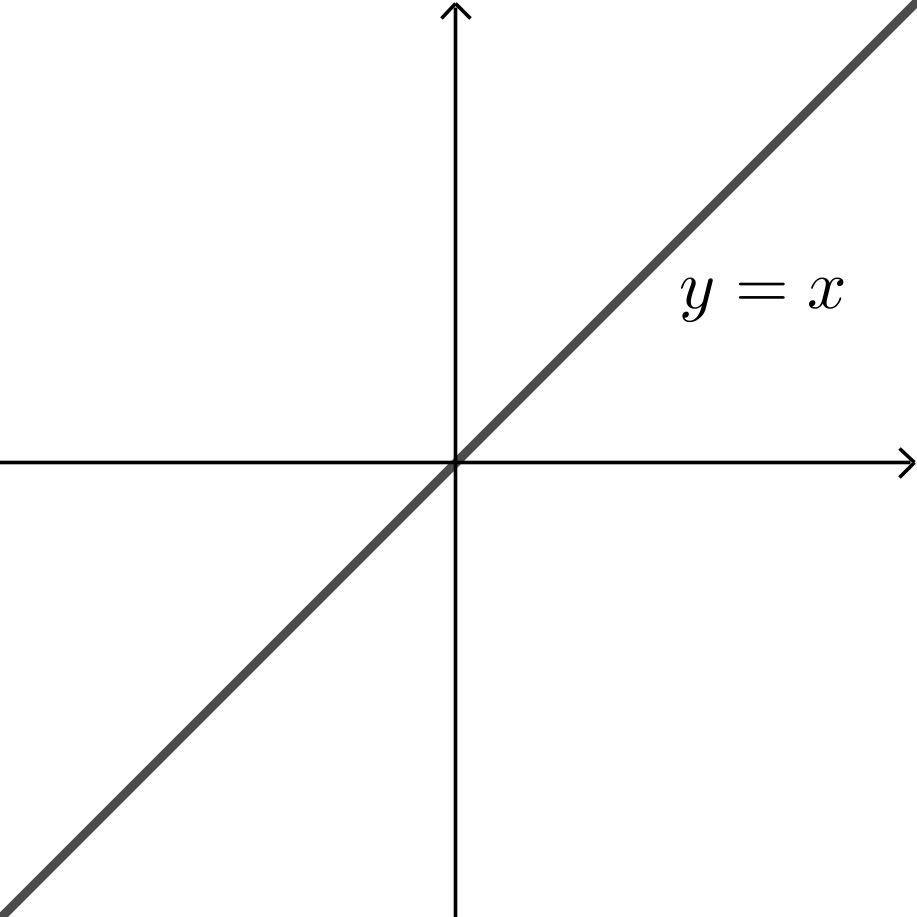
\includegraphics[width=0.25\textwidth]{various_10-1}\qquad
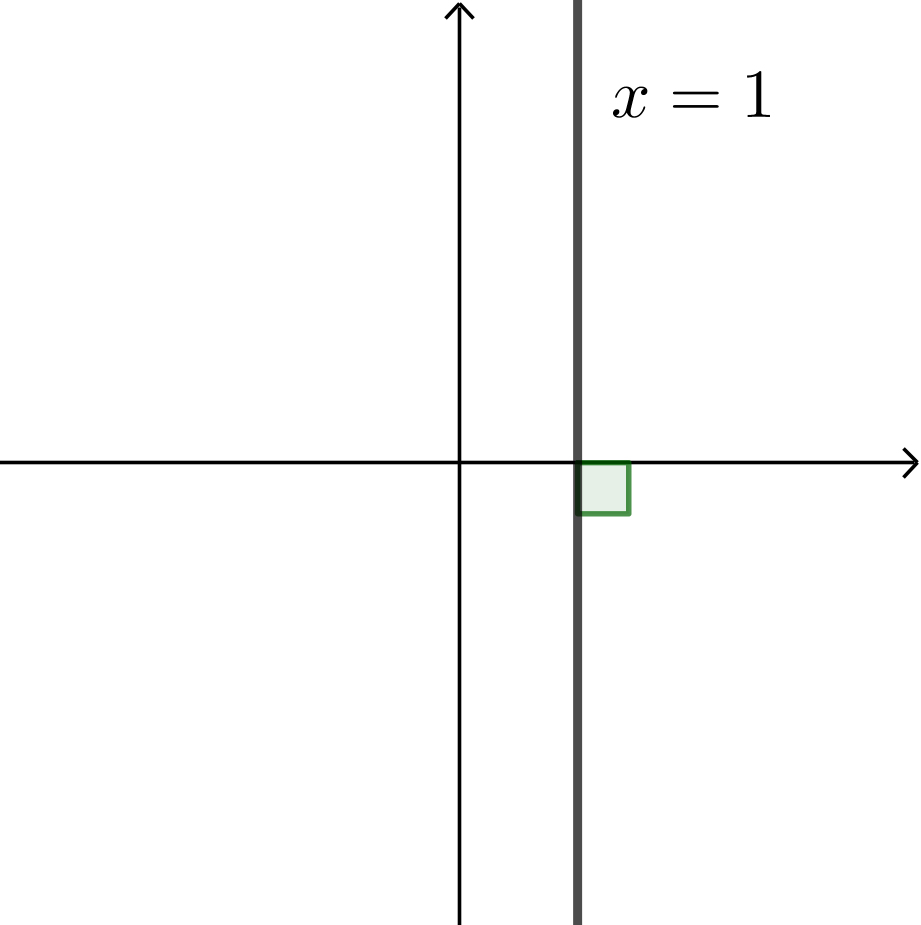
\includegraphics[width=0.25\textwidth]{various_10-2}\qquad
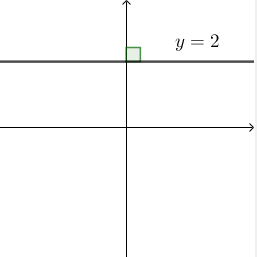
\includegraphics[width=0.25\textwidth]{various_10-3}
\end{center}



%%
\section{합성함수}
%
\exam{두 함수 \(f:X\to Y\), \(g:Y\to Z\)가 주어져 있을 때,}\label{composition1}
%\begin{enumerate}
%\item
%가 있다고 하자.
%즉 \(f\)의 공역과 \(g\)의 정의역이 일치한다.
\begin{center}
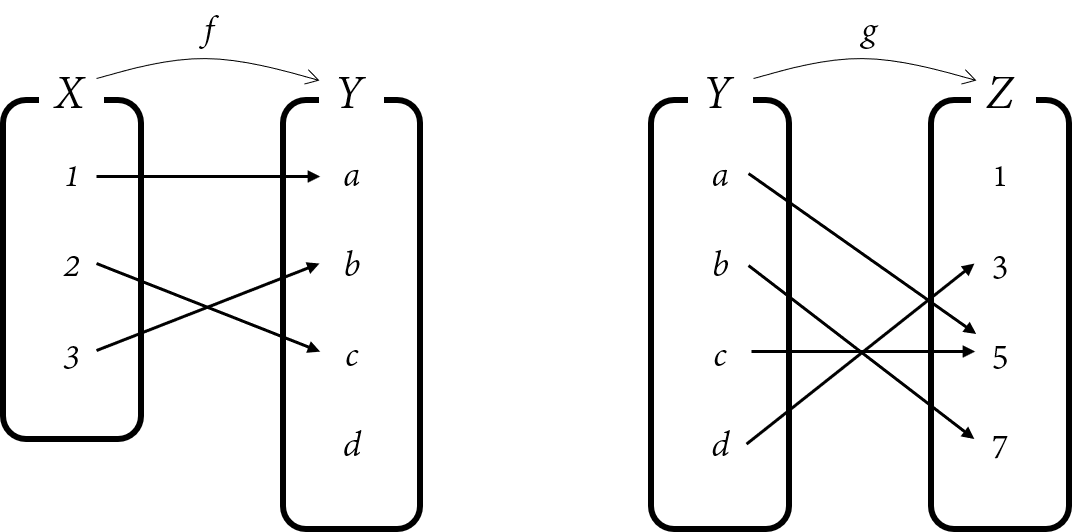
\includegraphics[width=0.5\textwidth]{composition_1-1}
\end{center}
%이런 경우에 두 함수를 합쳐서
새로운 함수 \(g\circ f:X\to Z\)를 다음과 같이 만들 수 있다.
\begin{center}
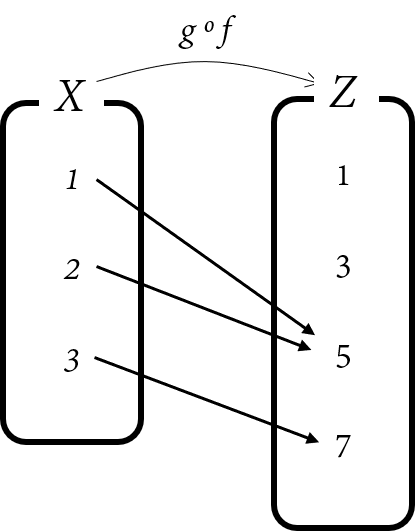
\includegraphics[width=0.2\textwidth]{composition_1-2}
\end{center}
%\item
%두 함수 \(f:X\to Y\), \(g:Y\to Z\)가 주어져 있을 때,
%%이번에는 \(f:X\to Y\)와 \(g:Z\to W\)로 주어졌다고 하자.
%%\(f\)의 공역과 \(g\)의 정의역이 일치하지 않는다.
%\begin{center}
%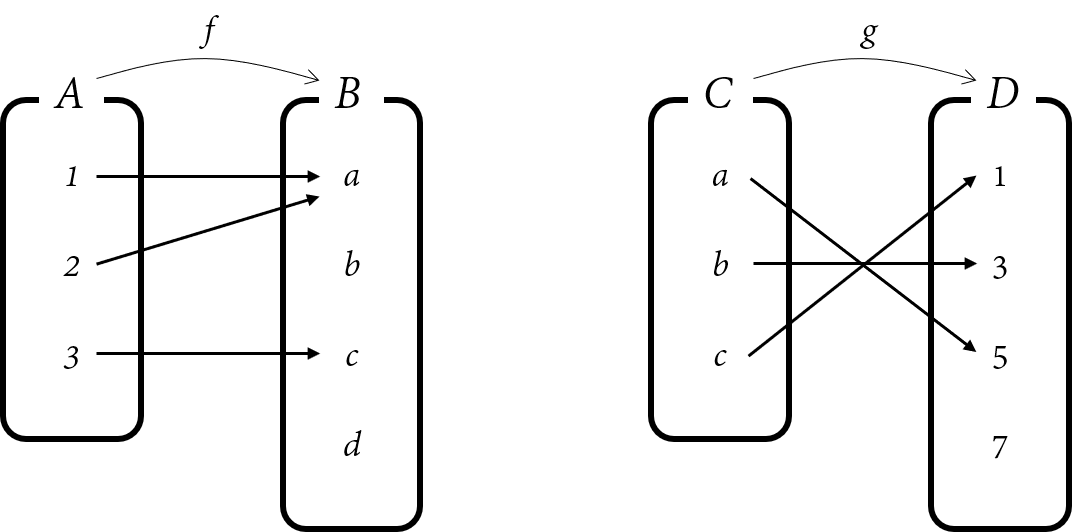
\includegraphics[width=0.5\textwidth]{composition_1-3}
%\end{center}
%새로운 함수 \(g\circ f:X\to W\)를 만들 수 있다.
%%이 경우에도 두 함수를 합쳐서 새로운 함수 \(g\circ f:X\to W\)를 만들 수 있다.
%\begin{center}
%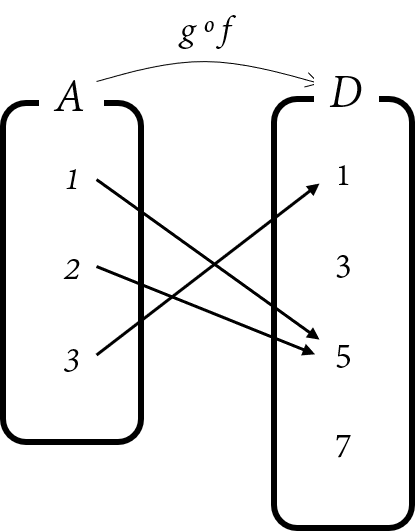
\includegraphics[width=0.2\textwidth]{composition_1-4}
%\end{center}
%\item
%두 함수 \(f:X\to Y\), \(g:Y\to Z\)가 주어져 있을 때,
%%이번에도 \(f\)의 공역과 \(g\)의 정의역이 일치하지 않도록 \(f:X\to Y\)와 \(g:Z\to W\)가 주어져있다고 하자.
%\begin{center}
%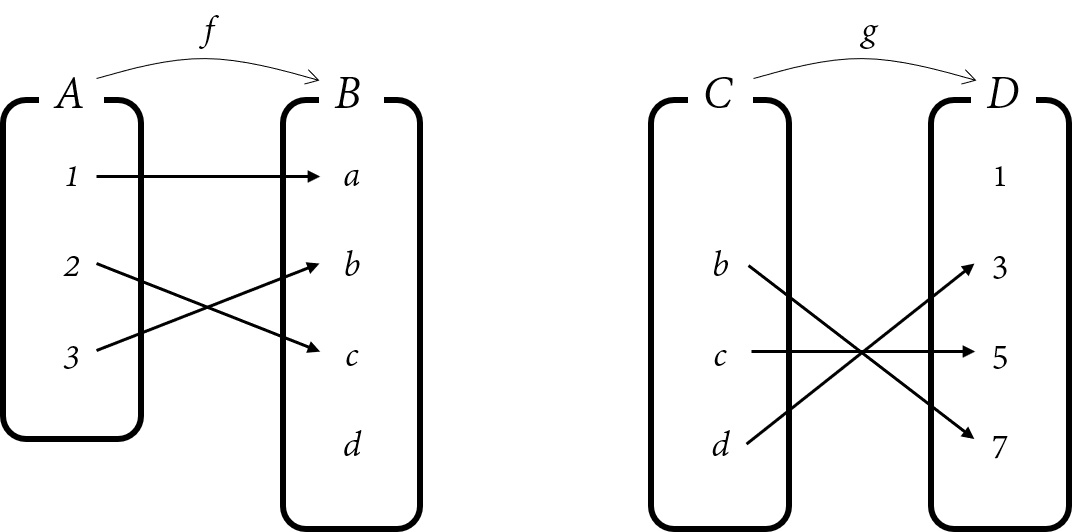
\includegraphics[width=0.5\textwidth]{composition_1-5}
%\end{center}
%새로운 대응 \(g\circ f:X\to W\)를 만들 수는 있지만 이것은 함수는 아니다.
%%이 경우에도 두 함수를 합쳐서 새로운 함수 \(g\circ f:X\to W\)를 만들 수 있다.
%\begin{center}
%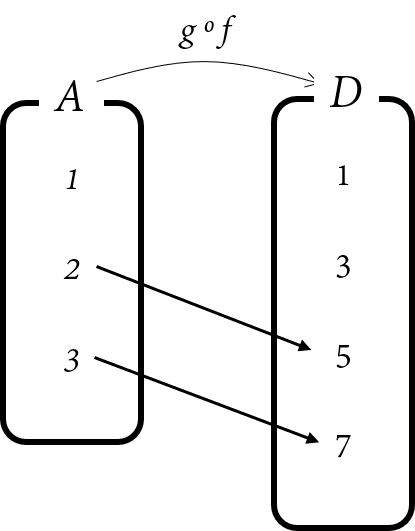
\includegraphics[width=0.2\textwidth]{composition_1-6}
%\end{center}
%\end{enumerate}

%이때 새로운 함수 \(g\circ f\)를 \(f\)와 \(g\)의 \fbox{합성함수}라고 부른다.
%\(f\)의 공역과 \(g\)의 정의역이 일치하는 (1)과 같은 경우에 합성함수가 잘 정의된다.
%\(f\)의 공역과 \(g\)의 정의역이 일치하지 않으면 (2)와 같이 합성함수가 잘 정의되는 경우도 있고 (3)과 같이 정의되지 않는 경우도 있다.

\begin{mdframed}
%
\defi{합성함수}\label{composition2}
%\begin{enumerate}
두 함수 \(f:X\to Y\), \(g:Y\to Z\)에 대하여 새로운 함수 \(g\circ f:X\to Z\)를
\[(g\circ f)(x)=g(f(x))\]
로 정의하자.
이 함수를 \(f\)와 \(g\)의 \fbox{합성함수}라고 부른다.
\end{mdframed}

%
\exam{예시 \ref{composition1})에서}\label{composition3}
\begin{align*}
(g\circ f)(1)&=g(f(1))=g(a)=5\\
(g\circ f)(2)&=g(f(2))=g(c)=5\\
(g\circ f)(3)&=g(f(3))=g(b)=7
\end{align*}

%
\prob{세 집합 \(X=\{1,2,3,4,5,6\}\), \(Y=\{1,2,3,4\}\), \(Z=\{1,2,3,4,5,6,7\}\)에 대하여 함수 \(f:X\to Y\), \(g:Y\to Z\)를}\label{composition4}
\begin{align*}
f(x)&=x\text{의 약수의 개수}\\
g(x)&=2x-1
\end{align*}
로 정의하자.
아래 그림의 화살표를 채우고 \((g\circ f)(3)\), \((g\circ f)(6)\)의 값을 각각 구하여라.
\begin{center}
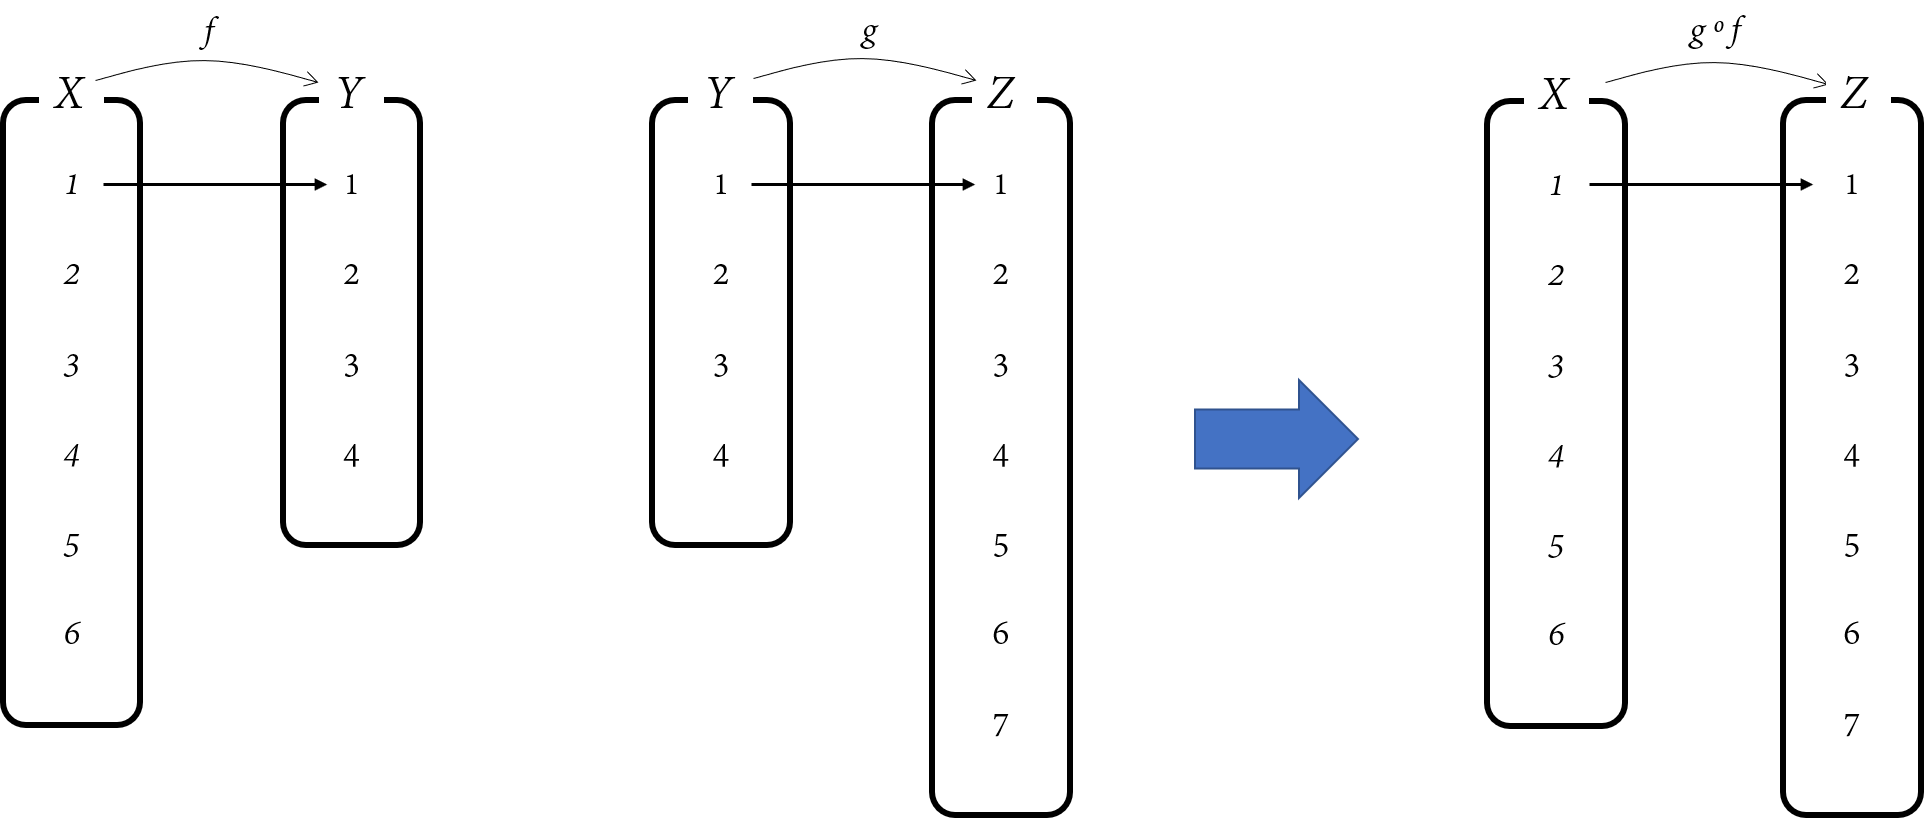
\includegraphics[width=0.8\textwidth]{composition_4}
\end{center}

%
\prob{두 함수 \(f\), \(g\)가}\label{composition5}
\[f(x)=2x-2,\qquad g(x)=x^2\]
로 정의될 때, \((g\circ f)(3)\)의 값을 구하여라.

\newpage
%
\exam{두 집합 \(X=\{1,2,3\}\), \(Y=\{a,b,c,d\}\)에 대하여 함수 \(f:X\to Y\)를}\label{composition6}
\[f(1)=a,\quad f(2)=c,\quad f(3)=d\]
로 정의하자.
%\(f(1)=a\), \(f(2)=c\), \(f(3)=d\)로 정의하자.
\(X\)의 항등함수 \(I_X\)에 대하여 \(f\circ I_X\)를 구하면,
\begin{center}
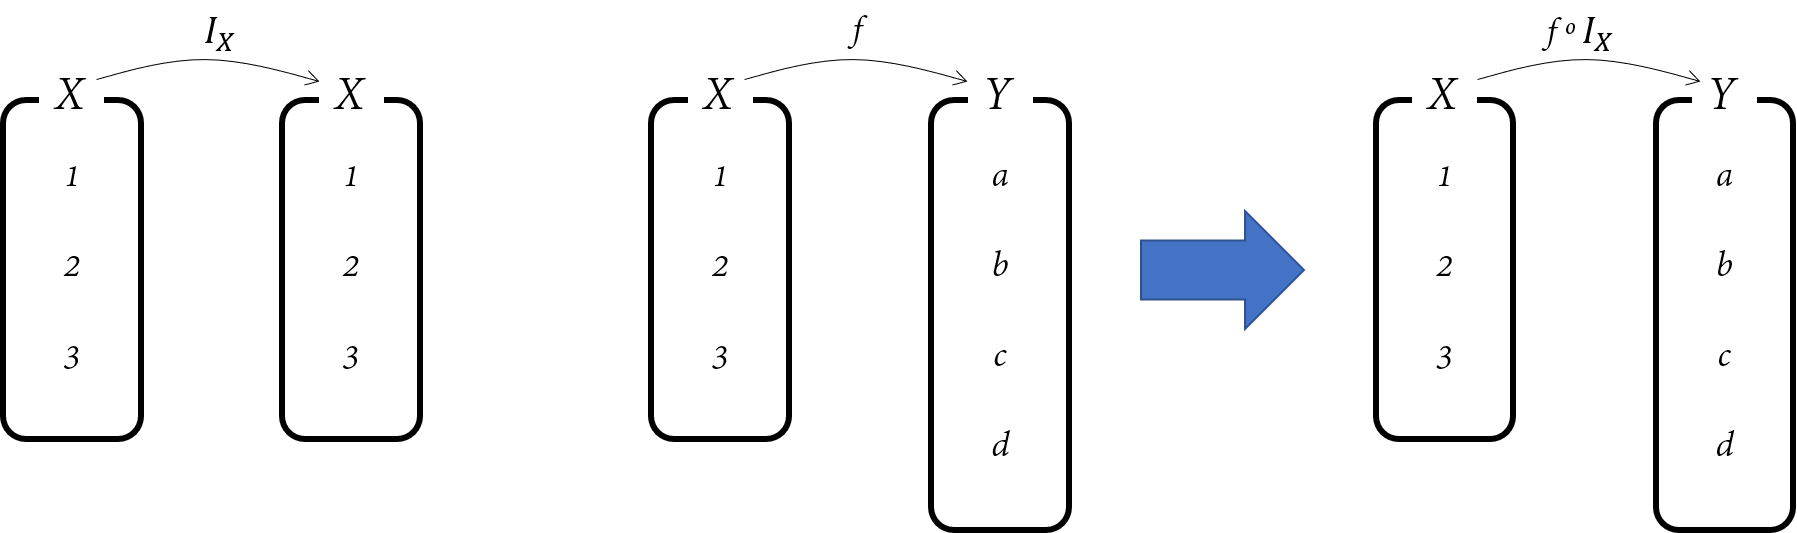
\includegraphics[width=0.9\textwidth]{composition_6-1}
\end{center}
이다.
따라서 \fbox{\(f\circ I_X=f\)}이다.
또 \(Y\)의 항등함수 \(I_Y\)에 대하여 \(I_Y\circ f\)를 구하면,
\begin{center}
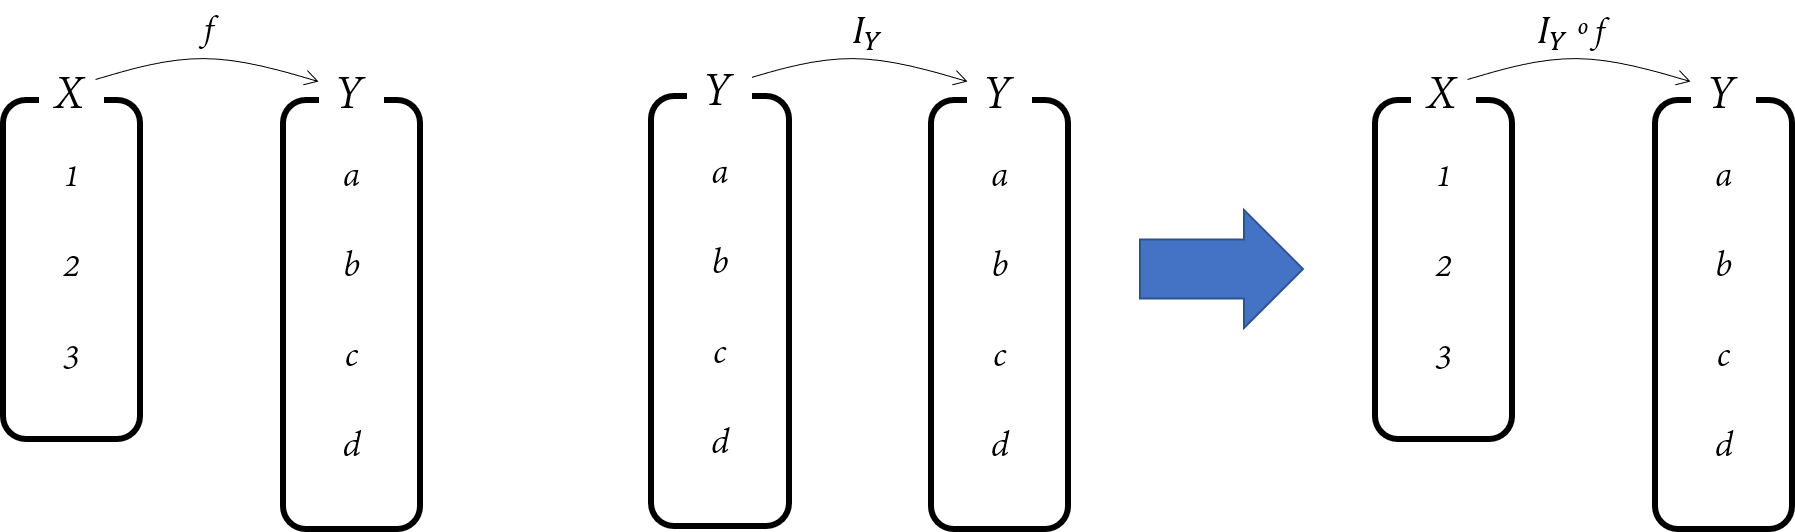
\includegraphics[width=0.9\textwidth]{composition_6-2}
\end{center}
이다.
따라서 \fbox{\(I_Y\circ f=f\)}이다.
%따라서,
%\begin{center}
%\fbox{\(f\circ I_X=I_Y\circ f=f\)}
%\end{center}
%이다.
%\(f\)의 정의역과 공역이 같은 경우에는 간단히
즉
\begin{center}
\fbox{\(f\circ I=I\circ f=f\)}
\end{center}
로 나타내기도 한다.

\bigskip
실수 \(a\)와 집합 \(A\)에 대하여
\begin{gather*}
a+0=0+a=a\\
a\times1=1\times a=a\\
A\cap U=U\cap A=A\\
A\cup\varnothing=\varnothing\cup A=A
\end{gather*}
인것과 비슷하다.

\newpage
%
\exam{집합 \(X=\{1,2,3\}\)에 대하여 함수 \(f:X\to X\), \(g:X\to X\)를}\label{composition7}
\begin{align*}
f(1)&=2,\qquad g(1)=1\\
f(2)&=3,\qquad g(2)=2\\
f(3)&=1,\qquad g(3)=2
\end{align*}
로 정의하자.
\(g\circ f\)를 구하면	
\begin{center}
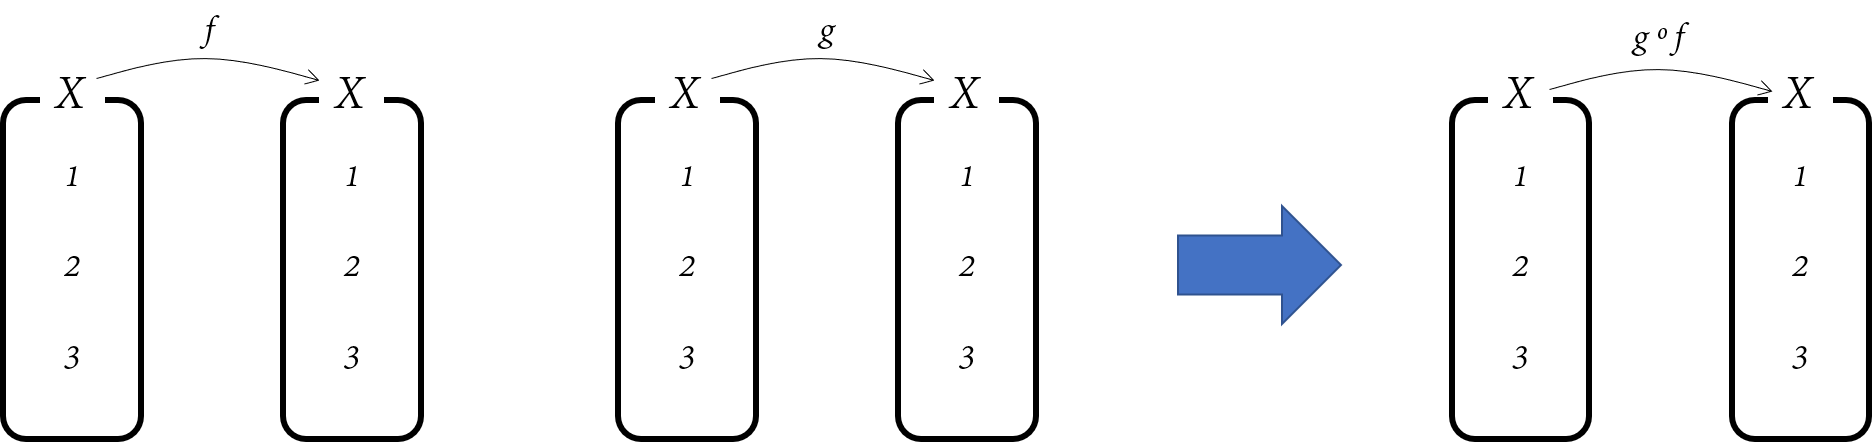
\includegraphics[width=0.9\textwidth]{composition_7-1}
\end{center}
이고, \(f\circ g\)를 구하면
\begin{center}
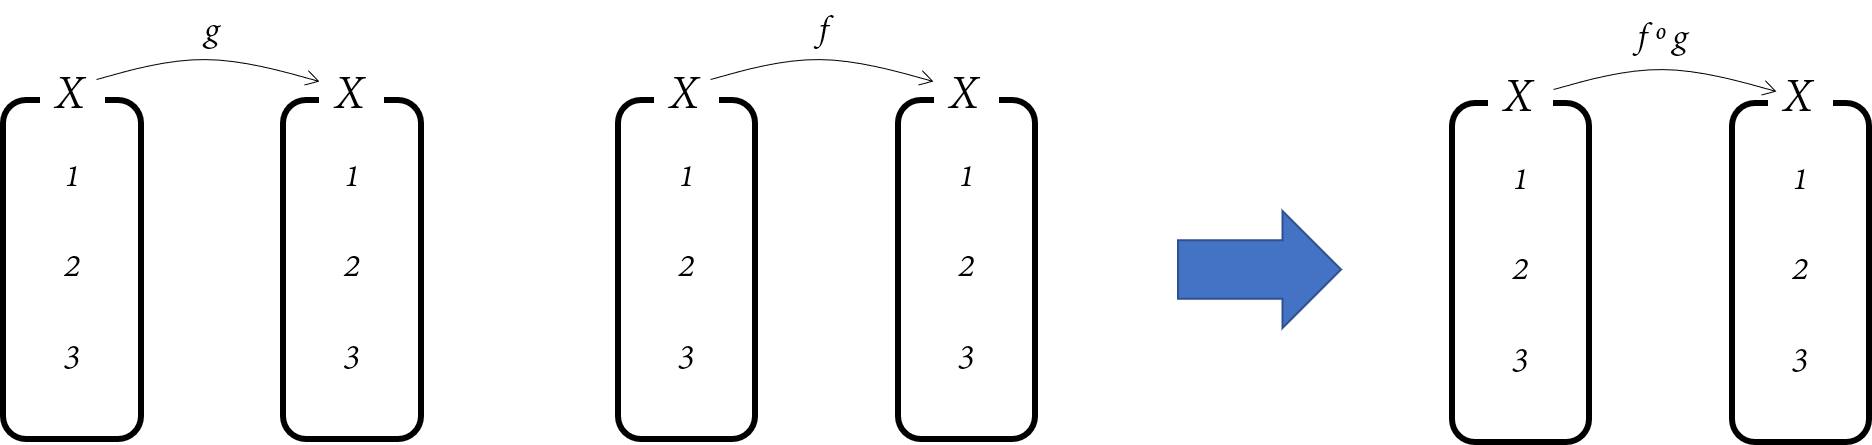
\includegraphics[width=0.9\textwidth]{composition_7-2}
\end{center}
이다.
따라서,
\begin{center}
\fbox{\(g\circ f\neq f\circ g\)}
\end{center}
이다.\footnotemark
\:\:
즉 함수의 합성에 대해서는 교환법칙이 성립하지 않는다.
\footnotetext{
가끔씩은 \(g\circ f=f\circ g\)인 경우도 있다.
하지만 일반적으로 \(g\circ f\)와 \(f\circ g\)는 서로 다르다.}%고 봐야 한다.}

\newpage
%
\exam{세 함수 \(f:X\to Y\), \(g:Y\to Z\), \(h:Z\to W\)가 아래와 같이 주어져있다고 하자.}\label{composition8}
\begin{center}
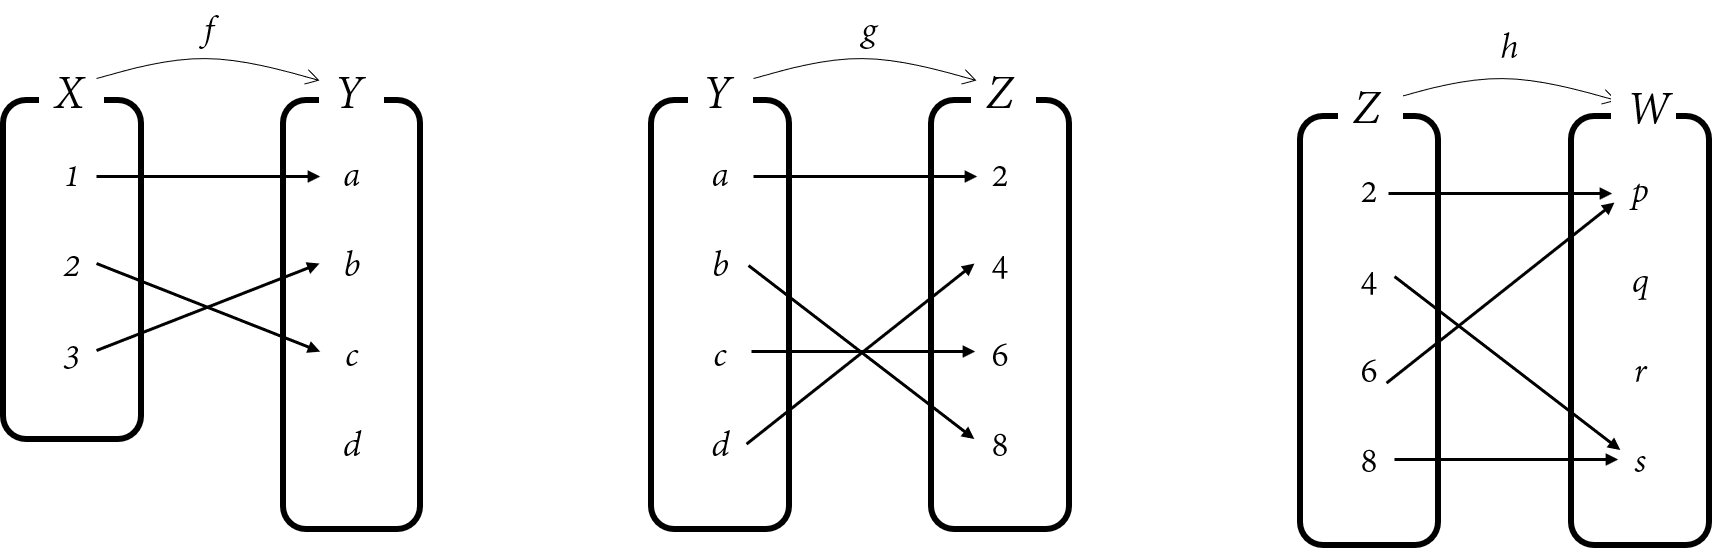
\includegraphics[width=0.9\textwidth]{composition_8}
\end{center}
\(((h\circ g)\circ f)(1)\)과 \((h\circ (g\circ f))(1)\)을 계산하면
\begin{align*}
((h\circ g)\circ f)(1)&=(h\circ g)(f(1))=(h\circ g)(a)=p\\
(h\circ (g\circ f))(1)&=h((g\circ f)(1))=h(2)=p
\end{align*}
이다.
따라서
\[((h\circ g)\circ f)(1)=p=(h\circ (g\circ f))(1)\]
마찬가지로
\begin{gather*}
((h\circ g)\circ f)(2)=\pb p=(h\circ (g\circ f))(2)\\
((h\circ g)\circ f)(3)=\pb p=(h\circ (g\circ f))(3)
\end{gather*}
이다.
그러므로
\begin{center}
\fbox{\((h\circ g)\circ f=h\circ(g\circ f)\)}
\end{center}
이다.
즉, 함수의 합성에 대해서 결합법칙이 성립한다.

\newpage
%예시 \ref{composition6}--\ref{composition8})을 종합하면,
%합성함수에 대하여 다음과 같은 성질들이 있다.
\begin{mdframed}
%
\theo{합성함수의 성질}
\begin{enumerate}[label=(\alph*)]\label{composition9}
\item
\(I\circ f=f\circ I=f\)
%\footnotemark
\item
\(g\circ f\neq f\circ g\)
\item
\((h\circ g)\circ f=h\circ(g\circ f)\)
\end{enumerate}
\end{mdframed}
%\footnotetext{
%좀 더 정확하게는,
%함수 \(f\)의 정의역이 \(X\)이고 공역이 \(Y\)일 때, 
%%\(f:X\to Y\)에 대하여
%\(I_X\circ f=f\circ I_Y=f\)이다.}

%
\prob{함수 \(f:X\to X\)가 다음과 같이 주어져있을 때,}\label{composition10}
\begin{center}
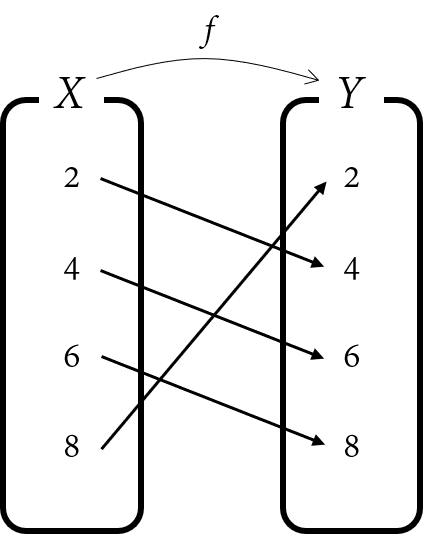
\includegraphics[width=0.2\textwidth]{composition_10-1}
\end{center}
\bigskip\bigskip
다음 함수들을 각각 구하여라.
\begin{flushleft}
%\begin{tabu}{X[c]X[c]X[c]}
\hspace{40pt}
(1) \(f\circ f\)
\hspace{50pt}
%&
(2) \(f\circ f\circ f\)
%&
\hspace{40pt}
(3) \(f\circ f\circ f\circ f\)
%\end{tabu}
\end{flushleft}
\begin{center}
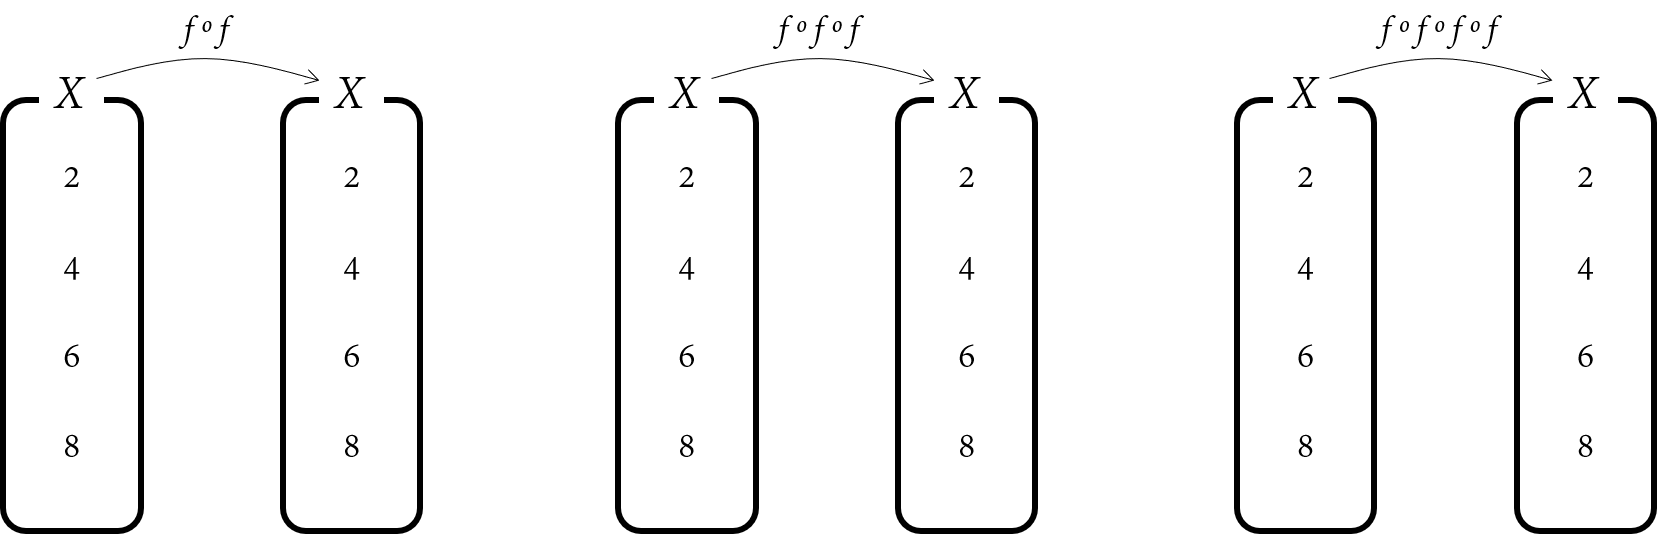
\includegraphics[width=0.8\textwidth]{composition_10-2}
\end{center}

%%
\section{역함수}
함수란, 모든 \(x\)값이 하나의 \(y\)값에 대응되는 것을 말했다.
또 일대일대응이란, 모든 \(y\)값들이 하나의 \(x\)값들로부터 대응되는 것을 말했다.
따라서 어떤 함수가 일대일대응이면, \(y\)를 \(x\)로 보내는 함수를 만들 수 있다.

%
\exam{일대일대응인 함수 \(f:X\to Y\)가 주어져있을 때,}\label{inverse1}
새로운 함수 \(f^{-1}:Y\to X\)를 다음과 같이 만들자.
\begin{center}
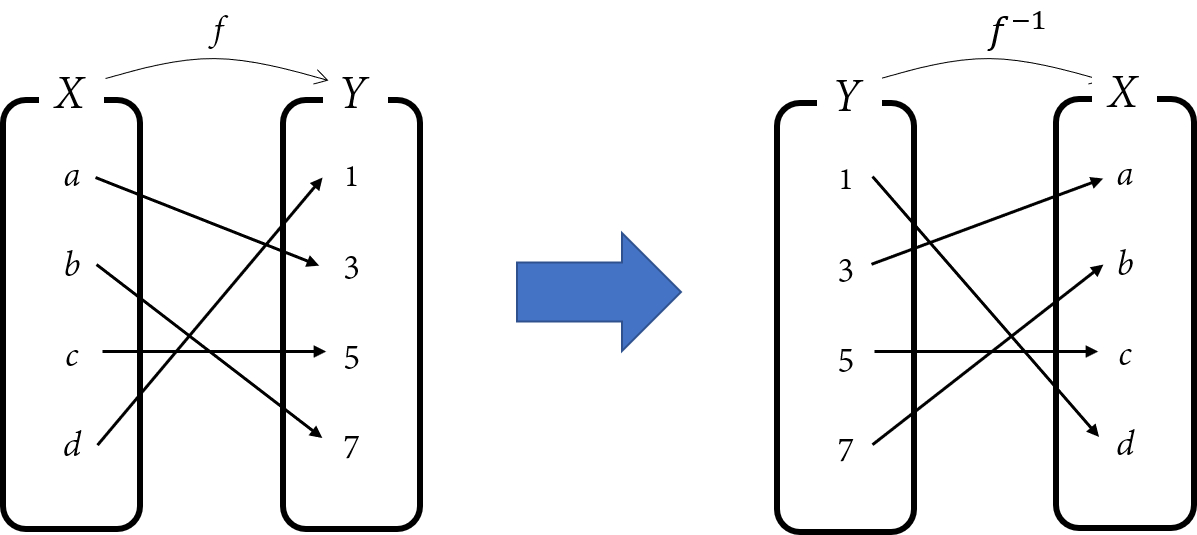
\includegraphics[width=0.6\textwidth]{inverse_1}
\end{center}
\(f(a)=3\)이기 때문에 \(f^{-1}(3)=a\)로 정했다.
마찬가지로
\begin{align*}
f(a)=3\qquad\Longrightarrow\qquad f^{-1}(3)=a\\
f(b)=7\qquad\Longrightarrow\qquad f^{-1}(7)=b\\
f(c)=5\qquad\Longrightarrow\qquad f^{-1}(5)=c\\
f(d)=1\qquad\Longrightarrow\qquad f^{-1}(1)=d
\end{align*}
이다.
이와 같은 함수 \(f^{-1}\)를 함수 \(f\)의 \fbox{역함수}라고 부르고 `\(f\) inverse'라고 읽는다.
\begin{mdframed}
%
\defi{역함수}\label{inverse2}
함수 \(f:X\to Y\)가 일대일대응일 때, \(f\)의 역함수 \(f^{-1}:Y\to X\)는
\[y=f(x)\iff x=f^{-1}(y)\]
를 만족시키는 함수이다.
\end{mdframed}

\newpage
%
\prob{주어진 함수 \(f\)의 역함수 \(f^{-1}\)를 화살표로 나타내어라.}\label{inverse3}
\begin{center}
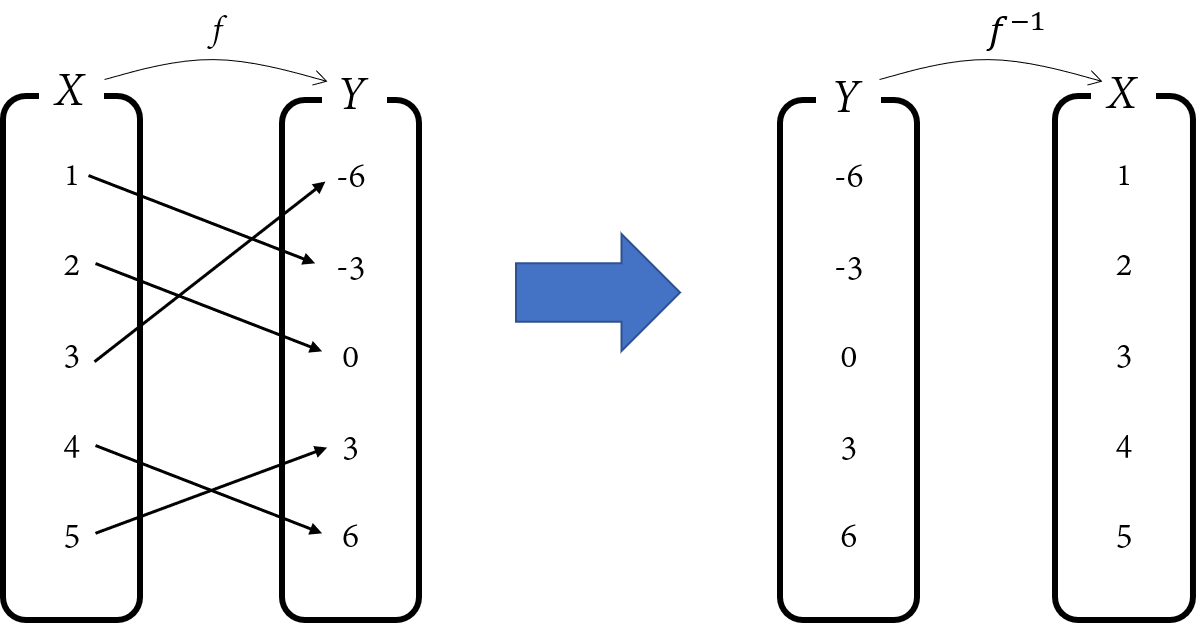
\includegraphics[width=0.5\textwidth]{inverse_3}
\end{center}
이때, \(f^{-1}(-6)=\pb{3}\), \(f^{-1}(6)=\pb{4}\)이다.


%
\prob{다음 세 함수 \(f\), \(g\), \(h\) 중 역함수가 존재하는 함수를 골라라.}\label{inverse4}
\begin{center}
(1)\hspace{100pt}(2)\hspace{100pt}(3)\\
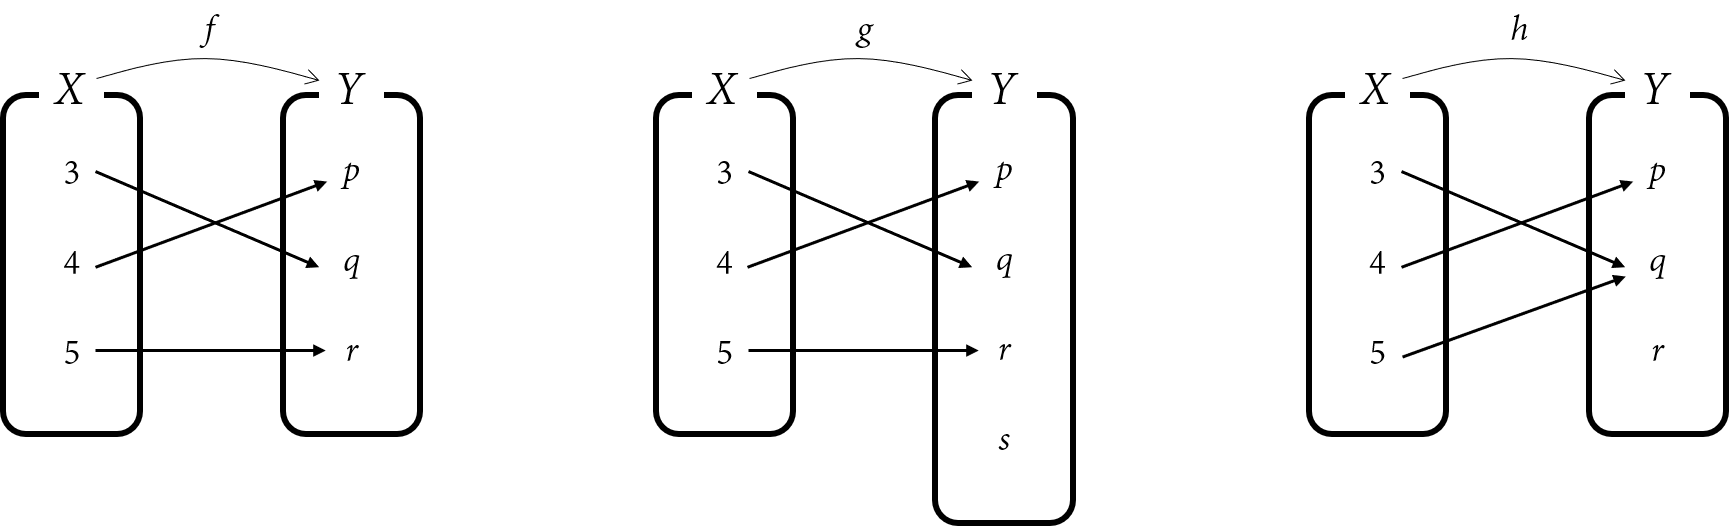
\includegraphics[width=0.8\textwidth]{inverse_4}
\end{center}

%
\prob{함수 \(f(x)=4x-1\)에 대하여 \(f^{-1}(7)=k\)일 때, 상수 \(k\)의 값을 구하여라.}\label{inverse5}

\newpage
%
\exam{함수 \(f(x)=2x-3\)의 역함수를 구하여라.}\label{inverse6}
\begin{mdframed}
정의역과 공역에 대한 말이 없으므로 정의역과 공역은 실수 전체의 집합이다.
따라서 역함수 \(f^{-1}\) 또한 정의역과 공역이 실수 전체의 집합이다.

%함수 \(f\)는, \(x\)를 \(y\)로 대응시키는 함수이고, 이때  \(y=2x-3\)이다.
%%\(y=2x-3\)이므로
%반면에, 함수 \(f^{-1}\)는 \(y\)를 \(x\)로 대응시키는 함수이다.

\(f\)는 \(x\)를 \(y\)로 대응시키는 함수이고, \(f^{-1}\)는 \(y\)를 \(x\)로 대응시키는 함수이다.
이때  \(y=2x-3\)이므로 \(x=\frac12(y+3)\)이다.
다시 말해, \(f^{-1}\)는 \(y\)를 \(\frac12(y+3)\)로 대응시키는 함수이다.
이것을 식으로 쓰면
\[f^{-1}(y)=\frac12(y+3)\]
이다.
%식 \(y=2x-3\)을 조금 변형하면 \(x=\frac12(y+3)\)이다.
%
%\(x\)값이 주어질 때, \(x\)는 \(y\)에 대응되었고 그때의 \(y\)값은 \(y=2x-3\)이었다.
%이제 \(y\)값이 주어지면, \(y\)는 \(x\)에 대응되고 그때의 \(x\)값은 \(x=\frac12(y+3)\)이다.
%즉 \(f^{-1}(y)=\frac12(y+3)\)이다.
이것을 간단히
\[f^{-1}(x)=\frac12(x+3)\]
로 쓰기도 한다.
즉 \(y=2x-3\)의 역함수는 \(y=\frac12(x+3)\)이다.
\end{mdframed}
\ans{\(f^{-1}(x)=\frac12(x+3)\)}

%
\prob{다음 함수들의 역함수를 구하여라.}\label{inverse7}
\begin{enumerate*}[itemjoin={\tabto{0.5\textwidth}}]
\item
\(f(x)=3x+3\)
\item
\(f(x)=-\frac12x+1\)
\end{enumerate*}

\newpage
%
\exam{}\label{inverse8}
예시 \ref{inverse6})에서 \(y=2x-3\)의 역함수는 \(y=\frac12(x+3)\)이다.
이것은
\[y=2x-3
\quad\xrightarrow{\phantom{x\:\leftarrow\: y,\:\: y\:\leftarrow\: x\:\:대입}}\quad
x=\frac12(y+3)
\quad\xrightarrow{x\:\leftarrow\: y,\:\: y\:\leftarrow\: x\:\:대입}\quad
y=\frac12(x+3)
\]
의 과정을 통해 구한 것이다.
즉 \(x\) 대신에 \(y\)를 대입하고, \(y\) 대신에 \(x\)를 대입하여 정리하면 역함수가 나온다.
따라서 \(y=f(x)\)의 그래프와 \(y=f^{-1}(x)\)의 그래프는 \(y=x\)에 대하여 대칭이다.
\begin{center}
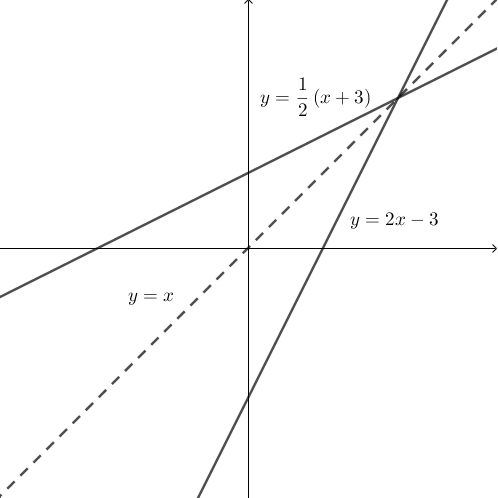
\includegraphics[width=0.5\textwidth]{inverse_6}
\end{center}

%
\prob{문제 \ref{inverse7})에서 함수와 역함수의 그래프들을 그려라.}\label{inverse9}
\begin{center}
(1)\hspace{130pt}(2)\\[10pt]
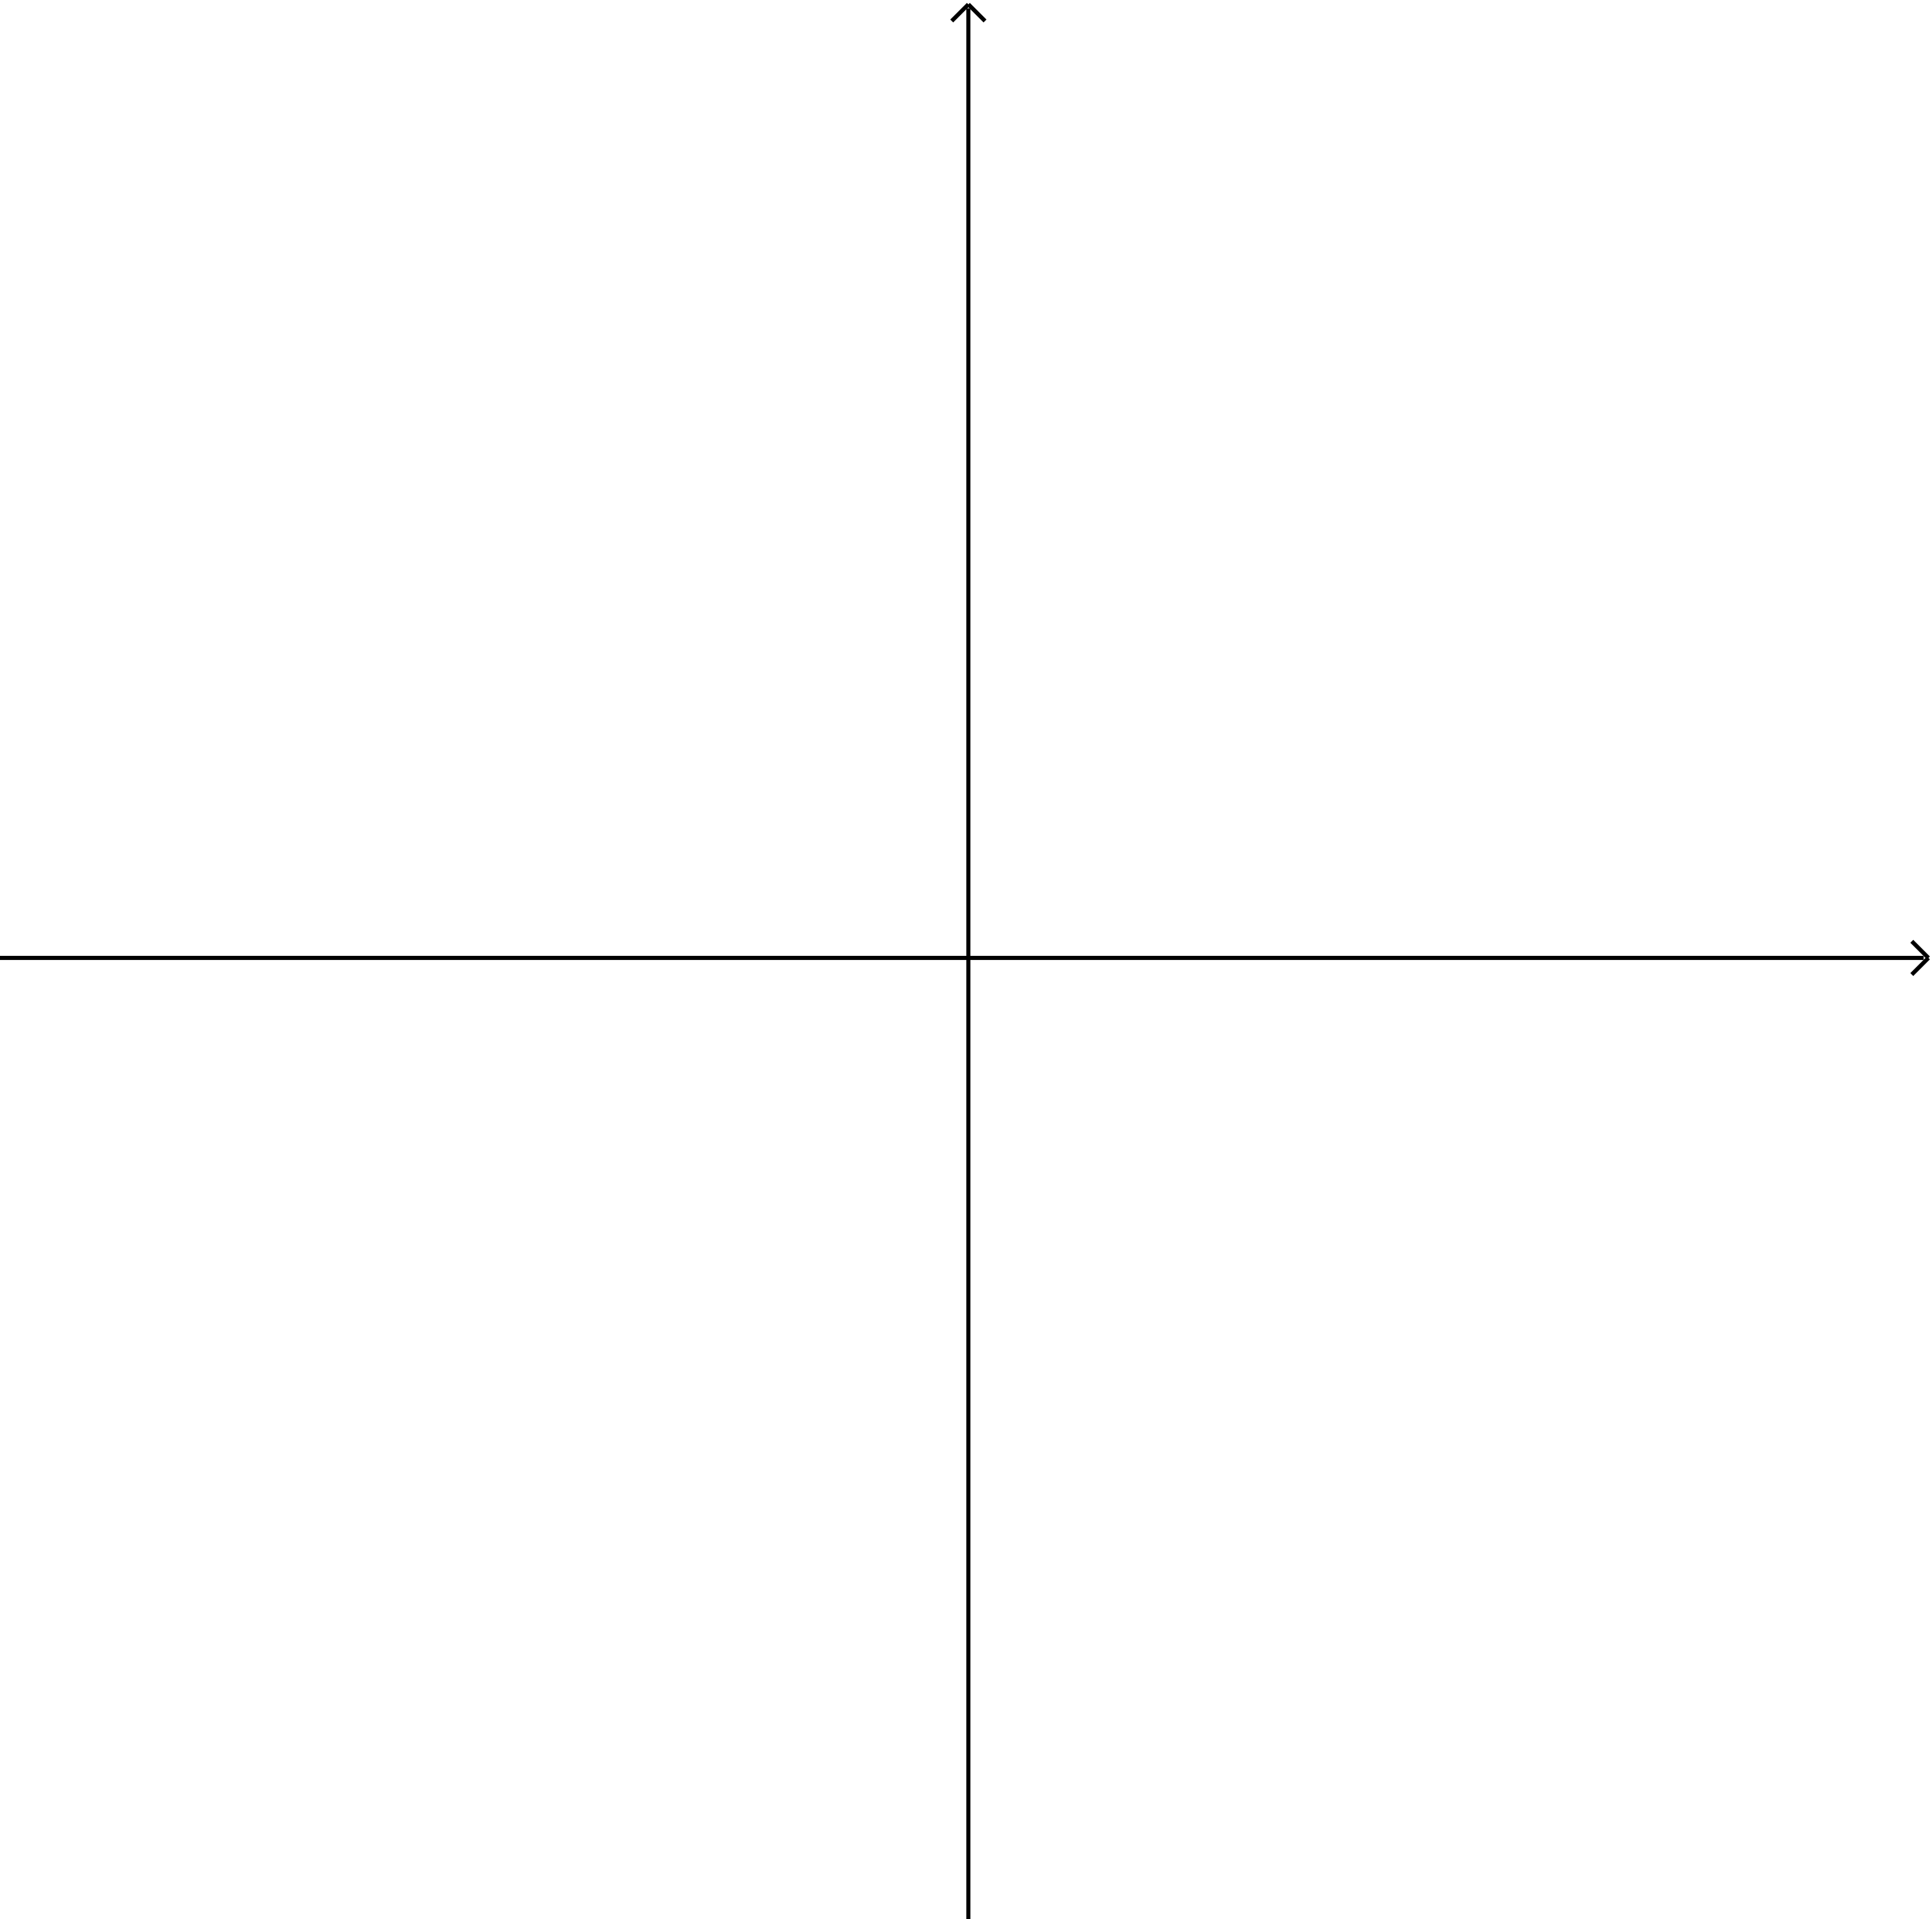
\includegraphics[width=0.4\textwidth]{xyaxes}~~
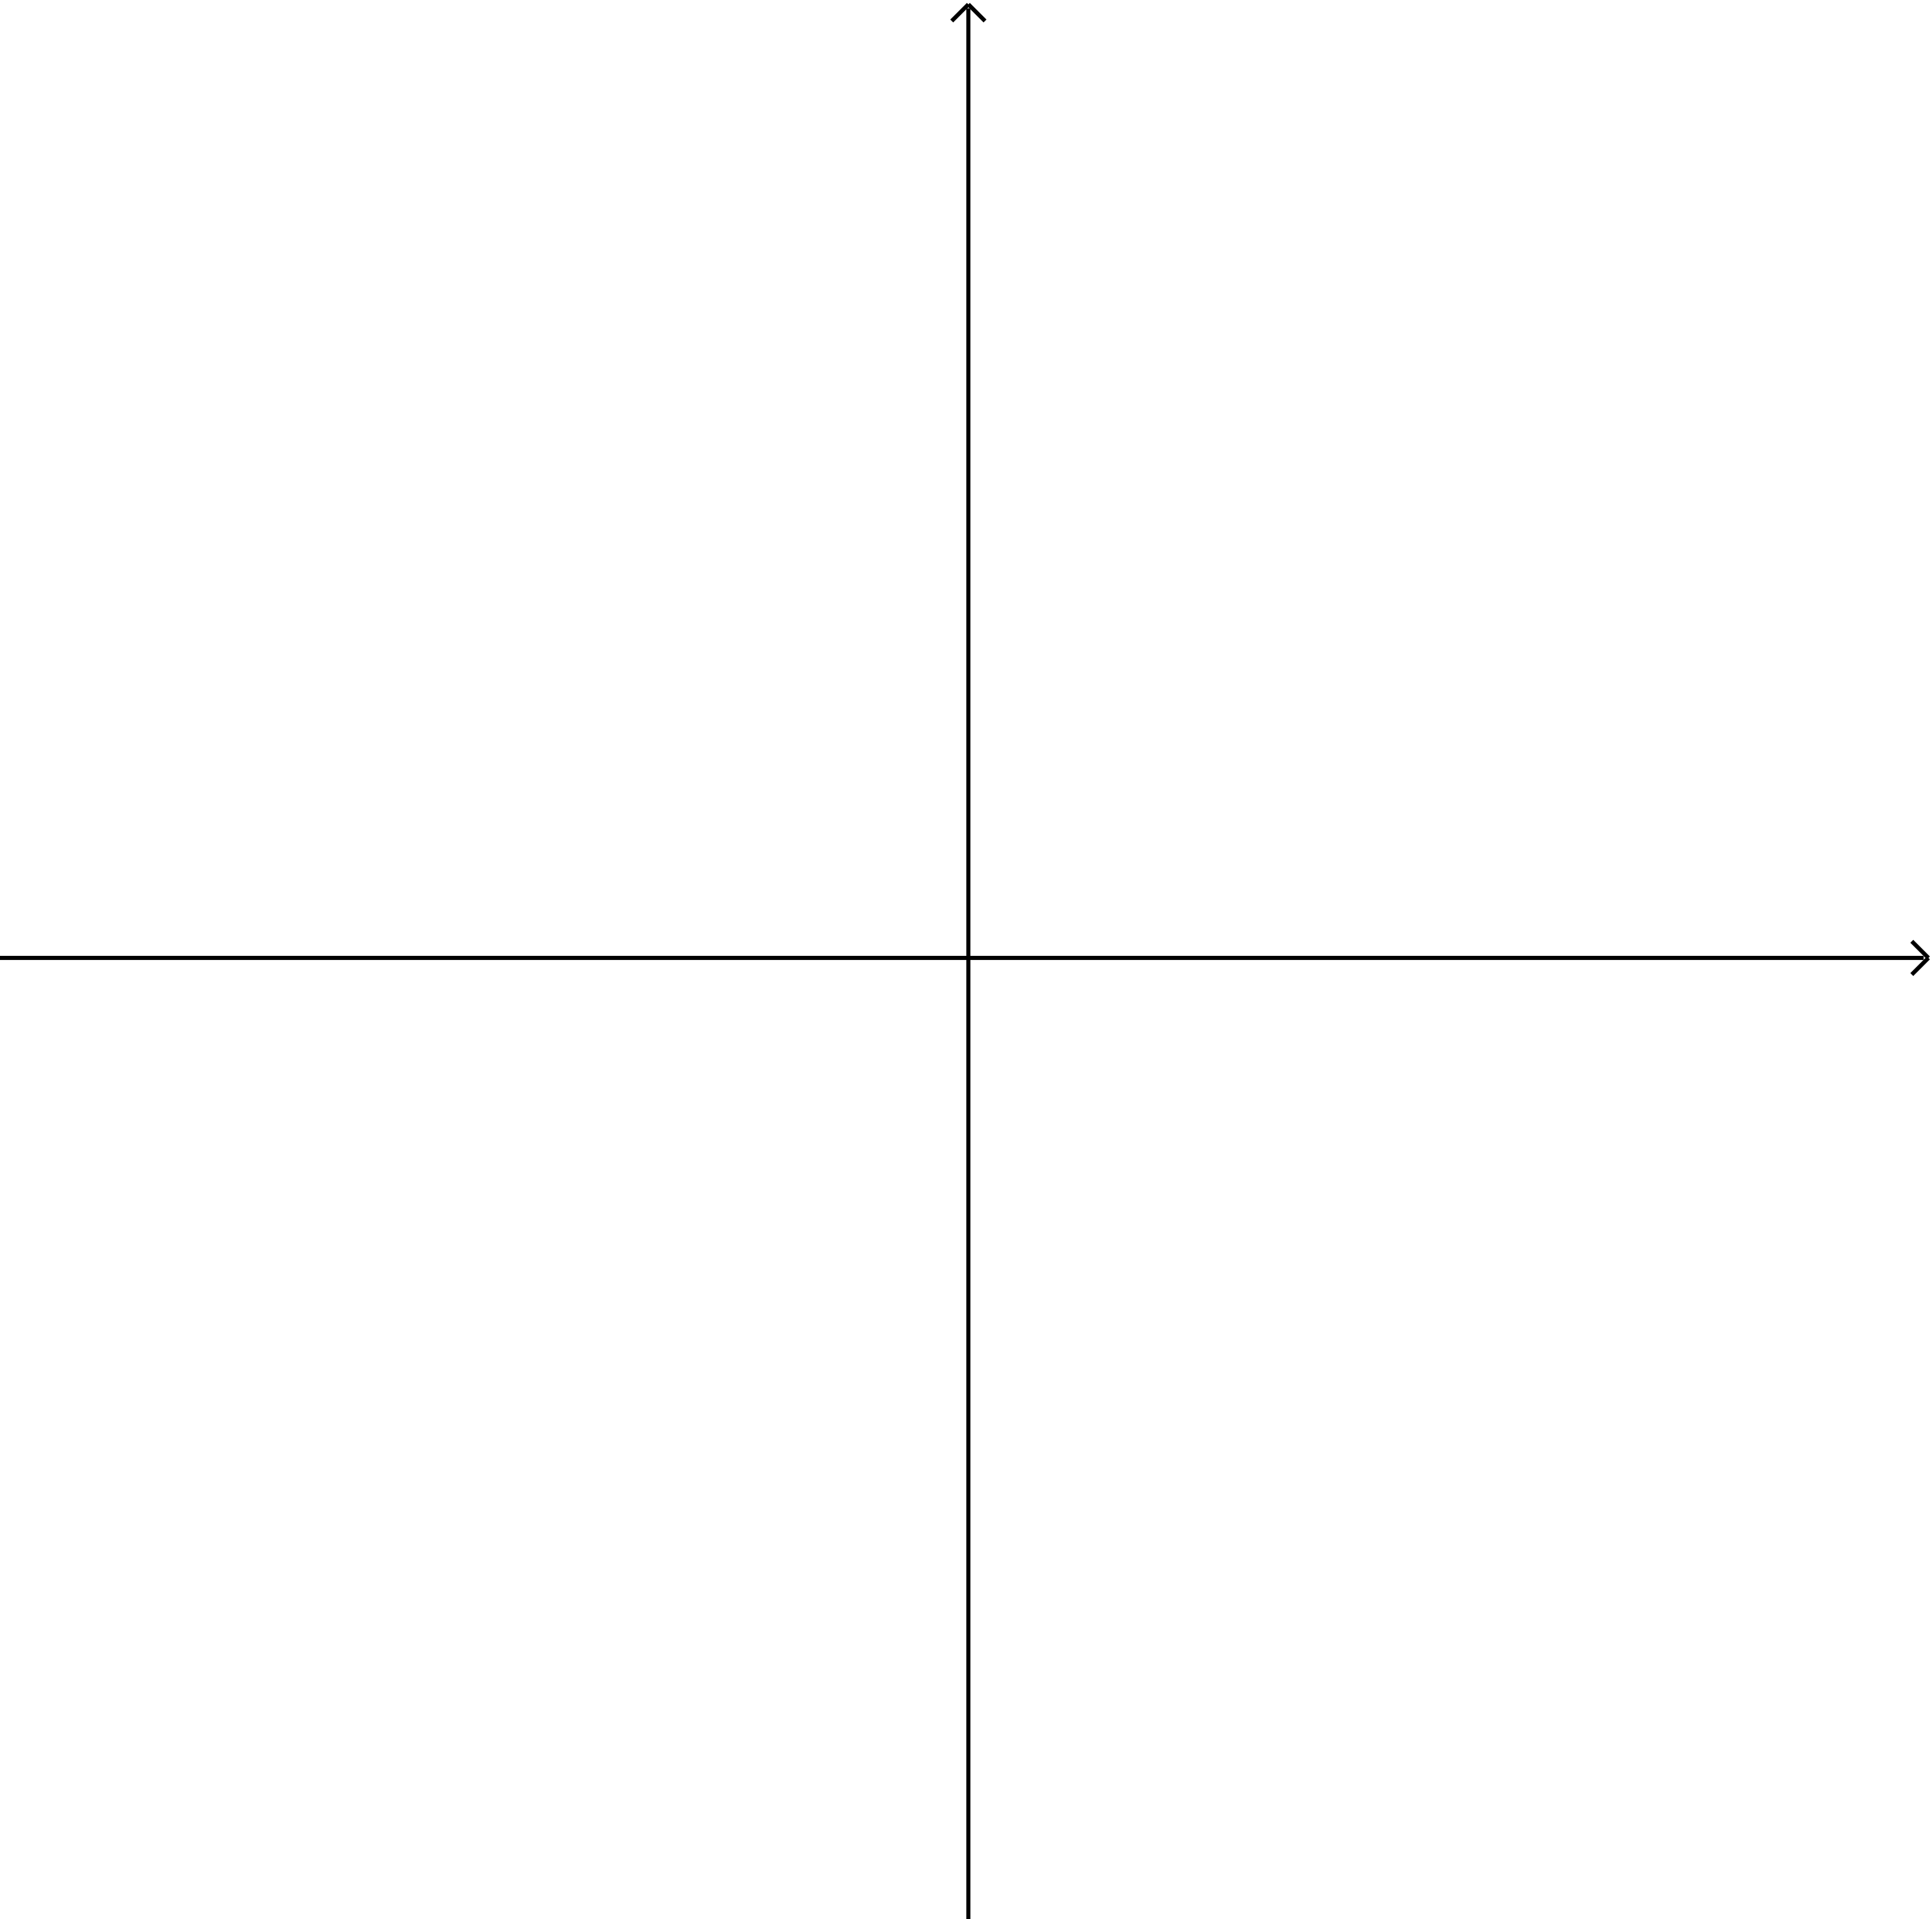
\includegraphics[width=0.4\textwidth]{xyaxes}
\end{center}


\newpage
%
\exam{항등함수 \(I\)의 역함수 \(I^{-1}\)을 구하면}\label{inverse10}
\vspace{-20pt}
\begin{center}
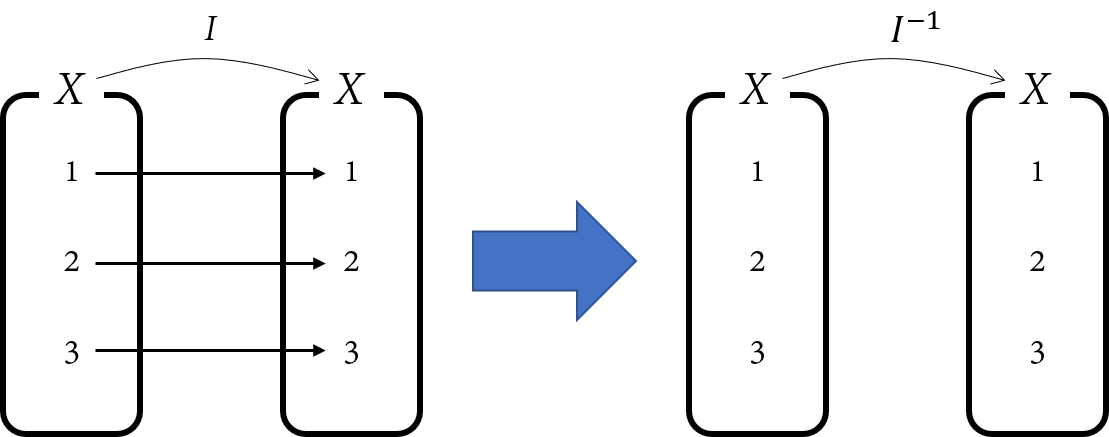
\includegraphics[width=0.5\textwidth]{inverse_10}
\end{center}
이다.
따라서
%\begin{center}
\fbox{\(I^{-1}=I\)}
%\end{center}
이다.

%
\exam{\(f\)의 역함수 \(f^{-1}\)를 구하고 다시 \(f^{-1}\)의 역함수 \((f^{-1})^{-1}\)를 구하면}\label{inverse11}
\vspace{-20pt}
\begin{center}
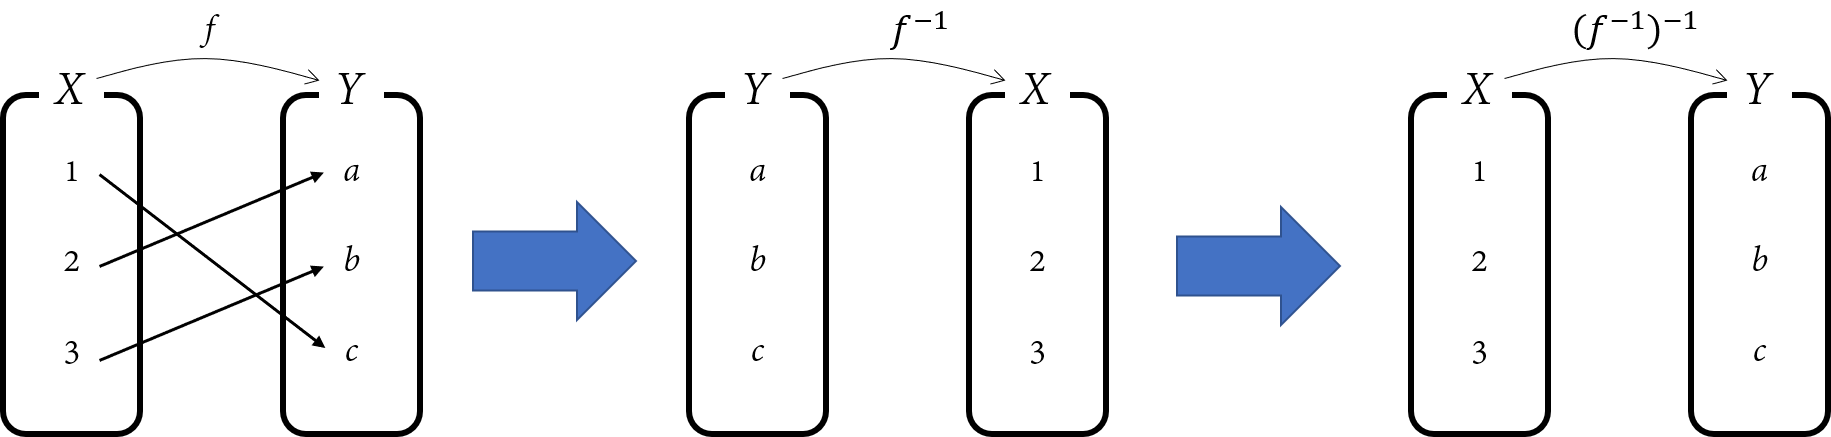
\includegraphics[width=0.8\textwidth]{inverse_11}
\end{center}
이다.
따라서
%\begin{center}
\fbox{\((f^{-1})^{-1}=f\)}
%\end{center}
이다.

%
\exam{함수 \(f:X\to Y\)에 대하여 \(f^{-1}\circ f\)를 구하면}\label{inverse12}
\vspace{-20pt}
\begin{center}
\includegraphics[width=0.8\textwidth]{inverse_12-1}
\end{center}
이다.
따라서
\fbox{\(f^{-1}\circ f=I_X\)}
이다.
또한, \(f\circ f^{-1}\)를 구하면
\begin{center}
\includegraphics[width=0.8\textwidth]{inverse_12-2}
\end{center}
이다.
따라서
\fbox{\(f\circ f^{-1}=I_Y\)}
이다.
이것들을 간단히
%\vspace{-20pt}
\begin{center}
\fbox{\(f^{-1}\circ f=f\circ f^{-1}=I\)}
\end{center}
라고 쓰기도 한다.

\newpage
%
\exam{\(f:X\to Y\)와 \(g:Y\to X\)가 일대일대응일 때 다음을 증명하여라.}\label{inverse13}
\begin{center}
\(f\circ g=I\)이면 \(g\)는 \(f\)의 역함수이다.
\end{center}
\begin{mdframed}
\(f\)가 일대일대응이므로 \(f^{-1}\)가 존재한다.
\[f\circ g=I\]의 양변에 \(f^{-1}\)를 왼쪽에 합성시키면\footnotemark
\begin{align*}
f^{-1}\circ f\circ g&=f^{-1}\circ I\\
I\circ g&=f^{-1}\circ I\\
g&=f^{-1}
\end{align*}
따라서 \(g\)는 \(f\)의 역함수이다.
\end{mdframed}
\footnotetext{
함수의 합성은 교환법칙을 만족시키지 않으므로 합성하는 함수를 같은 쪽에만 합성시킬 수 있다.
예를 들어, \(\square=\triangle\)가 주어져 있을 때 \(f\)를 왼쪽에 합성시켜
\(f\circ\square=f\circ\triangle\)을 얻을 수 있고, 오른쪽에 합성시켜 \(\square\circ f=\triangle\circ f\)를 얻을 수 있다.
하지만 \(\square\)에는 왼쪽에, \(\triangle\)에는 오른쪽에 합성시켜 \(f\circ\square=\triangle\circ f\)를 얻어낼 수는 없다.
}

%
\prob{\(f:X\to Y\)와 \(g:Y\to X\)가 일대일대응일 때 다음을 증명하여라.}\label{inverse14}
\begin{center}
\(g\circ f=I\)이면 \(g\)는 \(f\)의 역함수이다.
\end{center}

\newpage
%
\exam{두 함수 \(f:X\to Y\), \(g:Y\to Z\)가 일대일대응이고, 다음과 같이 주어졌다고 하자.}\label{inverse15}
\begin{center}
\includegraphics[width=0.4\textwidth]{inverse_15-1}
\end{center}
\(g\circ f:X\to Z\)는 일대일대응이므로 역함수 \((g\circ f)^{-1}:Z\to X\)가 존재한다.
\((g\circ f)(2)=6\)이므로 \((g\circ f)^{-1}(6)=2\)이어야 한다.
그리고 이것은
\[(g\circ f)^{-1}(6)=(f^{-1}\circ g^{-1})(6)=f^{-1}(g^{-1}(6))=f^{-1}(b)=2\]
와 같이 계산한 것과 같다.
\begin{center}
\includegraphics[width=0.4\textwidth]{inverse_15-2}
\end{center}
즉 \((g\circ f)^{-1}=g^{-1}\circ f^{-1}\)가 아니라
\begin{center}
\fbox{\((g\circ f)^{-1}=f^{-1}\circ g^{-1}\)}
\end{center}
이 성립한다.

\newpage
\begin{mdframed}
%
\theo{역함수의 성질}
\begin{enumerate}[label=(\alph*)]\label{inverse16}
\item
\(I^{-1}=I\)
\item
\((f^{-1})^{-1}=f\)
\item
\(f^{-1}\circ f=f\circ f^{-1}=I\)
\item
\(g=f^{-1}\iff f\circ g=I\iff g\circ f=I\)
\item
\((g\circ f)^{-1}=f^{-1}\circ g^{-1}\)
\end{enumerate}
\end{mdframed}

%
\prob{다음 중 \(f\circ f=I\)를 만족시키는 함수 \(f\)를 모두 골라라.}\label{inverse17}
\begin{center}
(1)\hspace{105pt}(2)\hspace{105pt}(3)\\
\includegraphics[width=0.9\textwidth]{inverse_17-1}\\[10pt]
(4)\hspace{105pt}(5)\hspace{105pt}(6)\\
\includegraphics[width=0.9\textwidth]{inverse_17-2}
\end{center}

%%
\section*{답}
\addcontentsline{toc}{chapter}{\protect\numberline{*}답}
\begin{multicols*}{2}

%
\ann{function3}{(1)}

%
\an{function4}
\begin{enumerate}
\item
\mbox{}\vtop{\vskip0pt \hbox{\includegraphics[width=0.2\textwidth]{function_4a}}}
%(1)\:\:\parbox[t]{0.8\columnwidth}{\includegraphics[width=0.2\textwidth]{function_3a}}
\item
정의역	$=\{1,2,3,4,5,6\}$\\
공역		$=\{1,2,3,4,5\}$\\
치역		$=\{1,2,3,4\}$
\end{enumerate}

%
\an{function5}
\(f(3)=3\), \(f(8)=0\), \(f(10)=2\)

%
\an{function7}
\begin{enumerate}
\item
정의역=실수 전체의 집합\\
공역=실수 전체의 집합\\
치역=정수 전체의 집합
\item
정의역=실수 전체의 집합\\
공역=실수 전체의 집합\\
치역=\(\{x\ba x\le3\}\)
\end{enumerate}

%
\an{function10}
\begin{enumerate*}[itemjoin=\qquad]
\item
같다
\item
다르다
\end{enumerate*}

%
\an{graph3}
\begin{center}
\includegraphics[width=\columnwidth]{graph_3a}
\end{center}

%
\ann{graph5}{(1), (3)}

%
\ann{various3}{\(a=5\), \(b=3\), \(c=2\)}
\begin{tabu}{>{\scriptsize}X[6,c]|X[c,$]X[c,$]X[c,$]X[c,$]X[c,$]X[c,$]}
			&(1)		&(2)		&(3)		&(4)		&(5)		&(6)		\\\hline
함수			&\bigcirc	&\bigcirc	&		&\bigcirc	&\bigcirc	&\bigcirc	\\
일대일함수	&\bigcirc	&\bigcirc	&		&		&\bigcirc	&		\\
일대일대응	&		&\bigcirc	&		&		&\bigcirc	&			
\end{tabu}

%
\ann{various5}{\(a=3\), \(b=2\), \(c=1\)}
\begin{tabu}{>{\scriptsize}X[5,c]|X[c,$]X[c,$]X[c,$]X[c,$]}
			&(1)		&(2)		&(3)		&(4)		\\\hline
함수			&\bigcirc	&\bigcirc	&		&\bigcirc	\\
일대일함수	&\bigcirc	&		&		&\bigcirc	\\
일대일대응	&\bigcirc	&		&		&		
\end{tabu}

%
\an{various8}
\begin{itemize}
\item
일대일함수이다
\item
일대일대응이다
\item
일대일함수가 아니다
\item
일대일대응이 아니다
\end{itemize}

%
\an{various9}
항등함수 : (1), 상수함수 : (3)

%
\ann{composition4}{\parbox[t]{0.6\columnwidth}{\((g\circ f)(3)=3\)\\ \((g\circ f)(6)=7\)}}
\begin{center}
\includegraphics[width=0.9\columnwidth]{composition_4a}
\end{center}

%
\ann{composition5}{\((g\circ f)(3)=16\)}

%
\an{composition10}
\begin{enumerate}
\item
\mbox{}\vtop{\vskip0pt \hbox{\includegraphics[width=0.4\columnwidth]{composition_10a-1}}}
\item
\mbox{}\vtop{\vskip0pt \hbox{\includegraphics[width=0.4\columnwidth]{composition_10a-2}}}
\item
\mbox{}\vtop{\vskip0pt \hbox{\includegraphics[width=0.4\columnwidth]{composition_10a-3}}}
\end{enumerate}

%
\ann{inverse3}{\(f^{-1}(-6)=3\), \(f^{-1}(6)=4\)}
\begin{center}
\includegraphics[width=0.4\columnwidth]{inverse_3a}
\end{center}

%
\ann{inverse4}{(1)}

%
\ann{inverse5}{\(k=2\)}
%\(f^{-1}(7)=k\)이므로 \(f(k)=7\), \(4k-1=7\), \(\therefore k=2\)

%
\an{inverse7}%{\parbox[t]{0.6\columnwidth}{\(f^{-1}(x)=\frac13(x-1)\)\\ \(f^{-1}(x)=-2x+5\)}}
\begin{enumerate}
\item
\(f^{-1}(x)=\frac13(x-3)\)
\item
\(f^{-1}(x)=-2x+2\)
\end{enumerate}

\newpage
%
\an{inverse9}
\begin{enumerate}
\item
\mbox{}\vtop{\vskip0pt \hbox{\includegraphics[width=0.7\columnwidth]{inverse_9a-1}}}
\item
\mbox{}\vtop{\vskip0pt \hbox{\includegraphics[width=0.7\columnwidth]{inverse_9a-2}}}
\end{enumerate}
%\begin{center}
%(1)\hspace{65pt}(2)\\[10pt]
%\includegraphics[width=0.4\columnwidth]{inverse_9a-1}~~
%\includegraphics[width=0.4\columnwidth]{inverse_9a-2}
%\end{center}

%
\an{inverse14}
\(f\)가 일대일대응이므로 \(f^{-1}\)가 존재한다.
\[f\circ g=I\]의 양변에 \(f^{-1}\)를 오른쪽에 합성시키면
\begin{align*}
g\circ f\circ f^{-1}&=I\circ f^{-1}\\
g\circ I&=I\circ f^{-1}\\
g&=f^{-1}
\end{align*}
따라서 \(g\)는 \(f\)의 역함수이다.

%
\ann{inverse17}{(1), (3), (4)}
\end{multicols*}

\newpage
\mbox{}
\newpage

%%
\section*{요약}
\addcontentsline{toc}{chapter}{\protect\numberline{*}요약}
\begin{enumerate}[label=\arabic*.,itemsep=15pt]
\item
함수
\begin{center}
\includegraphics[width=0.2\textwidth]{summary_1}
\end{center}
\item
함수의 그래프
\[\text{함수 \(f\)의 그래프}=\{(x,f(x))\ba x\in X\}\]
\item
여러가지 함수
\begin{itemize}
\item
\(함수
\quad\xrightarrow{x_1\neq x_2\Longrightarrow f(x_1)\neq f(x_2)}\quad
일대일함수
\quad\xrightarrow{공역=치역}\quad
일대일대응
\)
\item
항등함수 : \(f(x)=x\qquad(f=I)\)
\item
상수함수 : \(f(x)=c\qquad(c\text{는 상수})\)
\end{itemize}
\item
합성함수
\begin{center}
\includegraphics[width=0.8\textwidth]{summary_2}
\end{center}
\item
역함수
\begin{center}
\includegraphics[width=0.6\textwidth]{summary_3}
\end{center}
\end{enumerate}

\end{document}